\documentclass[11pt]{article}

    \usepackage[breakable]{tcolorbox}
    \usepackage{parskip} % Stop auto-indenting (to mimic markdown behaviour)
    
    \usepackage{iftex}
    \ifPDFTeX
    	\usepackage[T1]{fontenc}
    	\usepackage{mathpazo}
    \else
    	\usepackage{fontspec}
    \fi

    % Basic figure setup, for now with no caption control since it's done
    % automatically by Pandoc (which extracts ![](path) syntax from Markdown).
    \usepackage{graphicx}
    % Maintain compatibility with old templates. Remove in nbconvert 6.0
    \let\Oldincludegraphics\includegraphics
    % Ensure that by default, figures have no caption (until we provide a
    % proper Figure object with a Caption API and a way to capture that
    % in the conversion process - todo).
    \usepackage{caption}
    \DeclareCaptionFormat{nocaption}{}
    \captionsetup{format=nocaption,aboveskip=0pt,belowskip=0pt}

    \usepackage[Export]{adjustbox} % Used to constrain images to a maximum size
    \adjustboxset{max size={0.9\linewidth}{0.9\paperheight}}
    \usepackage{float}
    \floatplacement{figure}{H} % forces figures to be placed at the correct location
    \usepackage{xcolor} % Allow colors to be defined
    \usepackage{enumerate} % Needed for markdown enumerations to work
    \usepackage{geometry} % Used to adjust the document margins
    \usepackage{amsmath} % Equations
    \usepackage{amssymb} % Equations
    \usepackage{textcomp} % defines textquotesingle
    % Hack from http://tex.stackexchange.com/a/47451/13684:
    \AtBeginDocument{%
        \def\PYZsq{\textquotesingle}% Upright quotes in Pygmentized code
    }
    \usepackage{upquote} % Upright quotes for verbatim code
    \usepackage{eurosym} % defines \euro
    \usepackage[mathletters]{ucs} % Extended unicode (utf-8) support
    \usepackage{fancyvrb} % verbatim replacement that allows latex
    \usepackage{grffile} % extends the file name processing of package graphics 
                         % to support a larger range
    \makeatletter % fix for grffile with XeLaTeX
    \def\Gread@@xetex#1{%
      \IfFileExists{"\Gin@base".bb}%
      {\Gread@eps{\Gin@base.bb}}%
      {\Gread@@xetex@aux#1}%
    }
    \makeatother

    % The hyperref package gives us a pdf with properly built
    % internal navigation ('pdf bookmarks' for the table of contents,
    % internal cross-reference links, web links for URLs, etc.)
    \usepackage{hyperref}
    % The default LaTeX title has an obnoxious amount of whitespace. By default,
    % titling removes some of it. It also provides customization options.
    \usepackage{titling}
    \usepackage{longtable} % longtable support required by pandoc >1.10
    \usepackage{booktabs}  % table support for pandoc > 1.12.2
    \usepackage[inline]{enumitem} % IRkernel/repr support (it uses the enumerate* environment)
    \usepackage[normalem]{ulem} % ulem is needed to support strikethroughs (\sout)
                                % normalem makes italics be italics, not underlines
    \usepackage{mathrsfs}
    

    
    % Colors for the hyperref package
    \definecolor{urlcolor}{rgb}{0,.145,.698}
    \definecolor{linkcolor}{rgb}{.71,0.21,0.01}
    \definecolor{citecolor}{rgb}{.12,.54,.11}

    % ANSI colors
    \definecolor{ansi-black}{HTML}{3E424D}
    \definecolor{ansi-black-intense}{HTML}{282C36}
    \definecolor{ansi-red}{HTML}{E75C58}
    \definecolor{ansi-red-intense}{HTML}{B22B31}
    \definecolor{ansi-green}{HTML}{00A250}
    \definecolor{ansi-green-intense}{HTML}{007427}
    \definecolor{ansi-yellow}{HTML}{DDB62B}
    \definecolor{ansi-yellow-intense}{HTML}{B27D12}
    \definecolor{ansi-blue}{HTML}{208FFB}
    \definecolor{ansi-blue-intense}{HTML}{0065CA}
    \definecolor{ansi-magenta}{HTML}{D160C4}
    \definecolor{ansi-magenta-intense}{HTML}{A03196}
    \definecolor{ansi-cyan}{HTML}{60C6C8}
    \definecolor{ansi-cyan-intense}{HTML}{258F8F}
    \definecolor{ansi-white}{HTML}{C5C1B4}
    \definecolor{ansi-white-intense}{HTML}{A1A6B2}
    \definecolor{ansi-default-inverse-fg}{HTML}{FFFFFF}
    \definecolor{ansi-default-inverse-bg}{HTML}{000000}

    % commands and environments needed by pandoc snippets
    % extracted from the output of `pandoc -s`
    \providecommand{\tightlist}{%
      \setlength{\itemsep}{0pt}\setlength{\parskip}{0pt}}
    \DefineVerbatimEnvironment{Highlighting}{Verbatim}{commandchars=\\\{\}}
    % Add ',fontsize=\small' for more characters per line
    \newenvironment{Shaded}{}{}
    \newcommand{\KeywordTok}[1]{\textcolor[rgb]{0.00,0.44,0.13}{\textbf{{#1}}}}
    \newcommand{\DataTypeTok}[1]{\textcolor[rgb]{0.56,0.13,0.00}{{#1}}}
    \newcommand{\DecValTok}[1]{\textcolor[rgb]{0.25,0.63,0.44}{{#1}}}
    \newcommand{\BaseNTok}[1]{\textcolor[rgb]{0.25,0.63,0.44}{{#1}}}
    \newcommand{\FloatTok}[1]{\textcolor[rgb]{0.25,0.63,0.44}{{#1}}}
    \newcommand{\CharTok}[1]{\textcolor[rgb]{0.25,0.44,0.63}{{#1}}}
    \newcommand{\StringTok}[1]{\textcolor[rgb]{0.25,0.44,0.63}{{#1}}}
    \newcommand{\CommentTok}[1]{\textcolor[rgb]{0.38,0.63,0.69}{\textit{{#1}}}}
    \newcommand{\OtherTok}[1]{\textcolor[rgb]{0.00,0.44,0.13}{{#1}}}
    \newcommand{\AlertTok}[1]{\textcolor[rgb]{1.00,0.00,0.00}{\textbf{{#1}}}}
    \newcommand{\FunctionTok}[1]{\textcolor[rgb]{0.02,0.16,0.49}{{#1}}}
    \newcommand{\RegionMarkerTok}[1]{{#1}}
    \newcommand{\ErrorTok}[1]{\textcolor[rgb]{1.00,0.00,0.00}{\textbf{{#1}}}}
    \newcommand{\NormalTok}[1]{{#1}}
    
    % Additional commands for more recent versions of Pandoc
    \newcommand{\ConstantTok}[1]{\textcolor[rgb]{0.53,0.00,0.00}{{#1}}}
    \newcommand{\SpecialCharTok}[1]{\textcolor[rgb]{0.25,0.44,0.63}{{#1}}}
    \newcommand{\VerbatimStringTok}[1]{\textcolor[rgb]{0.25,0.44,0.63}{{#1}}}
    \newcommand{\SpecialStringTok}[1]{\textcolor[rgb]{0.73,0.40,0.53}{{#1}}}
    \newcommand{\ImportTok}[1]{{#1}}
    \newcommand{\DocumentationTok}[1]{\textcolor[rgb]{0.73,0.13,0.13}{\textit{{#1}}}}
    \newcommand{\AnnotationTok}[1]{\textcolor[rgb]{0.38,0.63,0.69}{\textbf{\textit{{#1}}}}}
    \newcommand{\CommentVarTok}[1]{\textcolor[rgb]{0.38,0.63,0.69}{\textbf{\textit{{#1}}}}}
    \newcommand{\VariableTok}[1]{\textcolor[rgb]{0.10,0.09,0.49}{{#1}}}
    \newcommand{\ControlFlowTok}[1]{\textcolor[rgb]{0.00,0.44,0.13}{\textbf{{#1}}}}
    \newcommand{\OperatorTok}[1]{\textcolor[rgb]{0.40,0.40,0.40}{{#1}}}
    \newcommand{\BuiltInTok}[1]{{#1}}
    \newcommand{\ExtensionTok}[1]{{#1}}
    \newcommand{\PreprocessorTok}[1]{\textcolor[rgb]{0.74,0.48,0.00}{{#1}}}
    \newcommand{\AttributeTok}[1]{\textcolor[rgb]{0.49,0.56,0.16}{{#1}}}
    \newcommand{\InformationTok}[1]{\textcolor[rgb]{0.38,0.63,0.69}{\textbf{\textit{{#1}}}}}
    \newcommand{\WarningTok}[1]{\textcolor[rgb]{0.38,0.63,0.69}{\textbf{\textit{{#1}}}}}
    
    
    % Define a nice break command that doesn't care if a line doesn't already
    % exist.
    \def\br{\hspace*{\fill} \\* }
    % Math Jax compatibility definitions
    \def\gt{>}
    \def\lt{<}
    \let\Oldtex\TeX
    \let\Oldlatex\LaTeX
    \renewcommand{\TeX}{\textrm{\Oldtex}}
    \renewcommand{\LaTeX}{\textrm{\Oldlatex}}
    % Document parameters
    % Document title
    \title{2021\_01\_13\_EE538\_Lecture2\_W2021}
    
    
    
    
    
% Pygments definitions
\makeatletter
\def\PY@reset{\let\PY@it=\relax \let\PY@bf=\relax%
    \let\PY@ul=\relax \let\PY@tc=\relax%
    \let\PY@bc=\relax \let\PY@ff=\relax}
\def\PY@tok#1{\csname PY@tok@#1\endcsname}
\def\PY@toks#1+{\ifx\relax#1\empty\else%
    \PY@tok{#1}\expandafter\PY@toks\fi}
\def\PY@do#1{\PY@bc{\PY@tc{\PY@ul{%
    \PY@it{\PY@bf{\PY@ff{#1}}}}}}}
\def\PY#1#2{\PY@reset\PY@toks#1+\relax+\PY@do{#2}}

\expandafter\def\csname PY@tok@w\endcsname{\def\PY@tc##1{\textcolor[rgb]{0.73,0.73,0.73}{##1}}}
\expandafter\def\csname PY@tok@c\endcsname{\let\PY@it=\textit\def\PY@tc##1{\textcolor[rgb]{0.25,0.50,0.50}{##1}}}
\expandafter\def\csname PY@tok@cp\endcsname{\def\PY@tc##1{\textcolor[rgb]{0.74,0.48,0.00}{##1}}}
\expandafter\def\csname PY@tok@k\endcsname{\let\PY@bf=\textbf\def\PY@tc##1{\textcolor[rgb]{0.00,0.50,0.00}{##1}}}
\expandafter\def\csname PY@tok@kp\endcsname{\def\PY@tc##1{\textcolor[rgb]{0.00,0.50,0.00}{##1}}}
\expandafter\def\csname PY@tok@kt\endcsname{\def\PY@tc##1{\textcolor[rgb]{0.69,0.00,0.25}{##1}}}
\expandafter\def\csname PY@tok@o\endcsname{\def\PY@tc##1{\textcolor[rgb]{0.40,0.40,0.40}{##1}}}
\expandafter\def\csname PY@tok@ow\endcsname{\let\PY@bf=\textbf\def\PY@tc##1{\textcolor[rgb]{0.67,0.13,1.00}{##1}}}
\expandafter\def\csname PY@tok@nb\endcsname{\def\PY@tc##1{\textcolor[rgb]{0.00,0.50,0.00}{##1}}}
\expandafter\def\csname PY@tok@nf\endcsname{\def\PY@tc##1{\textcolor[rgb]{0.00,0.00,1.00}{##1}}}
\expandafter\def\csname PY@tok@nc\endcsname{\let\PY@bf=\textbf\def\PY@tc##1{\textcolor[rgb]{0.00,0.00,1.00}{##1}}}
\expandafter\def\csname PY@tok@nn\endcsname{\let\PY@bf=\textbf\def\PY@tc##1{\textcolor[rgb]{0.00,0.00,1.00}{##1}}}
\expandafter\def\csname PY@tok@ne\endcsname{\let\PY@bf=\textbf\def\PY@tc##1{\textcolor[rgb]{0.82,0.25,0.23}{##1}}}
\expandafter\def\csname PY@tok@nv\endcsname{\def\PY@tc##1{\textcolor[rgb]{0.10,0.09,0.49}{##1}}}
\expandafter\def\csname PY@tok@no\endcsname{\def\PY@tc##1{\textcolor[rgb]{0.53,0.00,0.00}{##1}}}
\expandafter\def\csname PY@tok@nl\endcsname{\def\PY@tc##1{\textcolor[rgb]{0.63,0.63,0.00}{##1}}}
\expandafter\def\csname PY@tok@ni\endcsname{\let\PY@bf=\textbf\def\PY@tc##1{\textcolor[rgb]{0.60,0.60,0.60}{##1}}}
\expandafter\def\csname PY@tok@na\endcsname{\def\PY@tc##1{\textcolor[rgb]{0.49,0.56,0.16}{##1}}}
\expandafter\def\csname PY@tok@nt\endcsname{\let\PY@bf=\textbf\def\PY@tc##1{\textcolor[rgb]{0.00,0.50,0.00}{##1}}}
\expandafter\def\csname PY@tok@nd\endcsname{\def\PY@tc##1{\textcolor[rgb]{0.67,0.13,1.00}{##1}}}
\expandafter\def\csname PY@tok@s\endcsname{\def\PY@tc##1{\textcolor[rgb]{0.73,0.13,0.13}{##1}}}
\expandafter\def\csname PY@tok@sd\endcsname{\let\PY@it=\textit\def\PY@tc##1{\textcolor[rgb]{0.73,0.13,0.13}{##1}}}
\expandafter\def\csname PY@tok@si\endcsname{\let\PY@bf=\textbf\def\PY@tc##1{\textcolor[rgb]{0.73,0.40,0.53}{##1}}}
\expandafter\def\csname PY@tok@se\endcsname{\let\PY@bf=\textbf\def\PY@tc##1{\textcolor[rgb]{0.73,0.40,0.13}{##1}}}
\expandafter\def\csname PY@tok@sr\endcsname{\def\PY@tc##1{\textcolor[rgb]{0.73,0.40,0.53}{##1}}}
\expandafter\def\csname PY@tok@ss\endcsname{\def\PY@tc##1{\textcolor[rgb]{0.10,0.09,0.49}{##1}}}
\expandafter\def\csname PY@tok@sx\endcsname{\def\PY@tc##1{\textcolor[rgb]{0.00,0.50,0.00}{##1}}}
\expandafter\def\csname PY@tok@m\endcsname{\def\PY@tc##1{\textcolor[rgb]{0.40,0.40,0.40}{##1}}}
\expandafter\def\csname PY@tok@gh\endcsname{\let\PY@bf=\textbf\def\PY@tc##1{\textcolor[rgb]{0.00,0.00,0.50}{##1}}}
\expandafter\def\csname PY@tok@gu\endcsname{\let\PY@bf=\textbf\def\PY@tc##1{\textcolor[rgb]{0.50,0.00,0.50}{##1}}}
\expandafter\def\csname PY@tok@gd\endcsname{\def\PY@tc##1{\textcolor[rgb]{0.63,0.00,0.00}{##1}}}
\expandafter\def\csname PY@tok@gi\endcsname{\def\PY@tc##1{\textcolor[rgb]{0.00,0.63,0.00}{##1}}}
\expandafter\def\csname PY@tok@gr\endcsname{\def\PY@tc##1{\textcolor[rgb]{1.00,0.00,0.00}{##1}}}
\expandafter\def\csname PY@tok@ge\endcsname{\let\PY@it=\textit}
\expandafter\def\csname PY@tok@gs\endcsname{\let\PY@bf=\textbf}
\expandafter\def\csname PY@tok@gp\endcsname{\let\PY@bf=\textbf\def\PY@tc##1{\textcolor[rgb]{0.00,0.00,0.50}{##1}}}
\expandafter\def\csname PY@tok@go\endcsname{\def\PY@tc##1{\textcolor[rgb]{0.53,0.53,0.53}{##1}}}
\expandafter\def\csname PY@tok@gt\endcsname{\def\PY@tc##1{\textcolor[rgb]{0.00,0.27,0.87}{##1}}}
\expandafter\def\csname PY@tok@err\endcsname{\def\PY@bc##1{\setlength{\fboxsep}{0pt}\fcolorbox[rgb]{1.00,0.00,0.00}{1,1,1}{\strut ##1}}}
\expandafter\def\csname PY@tok@kc\endcsname{\let\PY@bf=\textbf\def\PY@tc##1{\textcolor[rgb]{0.00,0.50,0.00}{##1}}}
\expandafter\def\csname PY@tok@kd\endcsname{\let\PY@bf=\textbf\def\PY@tc##1{\textcolor[rgb]{0.00,0.50,0.00}{##1}}}
\expandafter\def\csname PY@tok@kn\endcsname{\let\PY@bf=\textbf\def\PY@tc##1{\textcolor[rgb]{0.00,0.50,0.00}{##1}}}
\expandafter\def\csname PY@tok@kr\endcsname{\let\PY@bf=\textbf\def\PY@tc##1{\textcolor[rgb]{0.00,0.50,0.00}{##1}}}
\expandafter\def\csname PY@tok@bp\endcsname{\def\PY@tc##1{\textcolor[rgb]{0.00,0.50,0.00}{##1}}}
\expandafter\def\csname PY@tok@fm\endcsname{\def\PY@tc##1{\textcolor[rgb]{0.00,0.00,1.00}{##1}}}
\expandafter\def\csname PY@tok@vc\endcsname{\def\PY@tc##1{\textcolor[rgb]{0.10,0.09,0.49}{##1}}}
\expandafter\def\csname PY@tok@vg\endcsname{\def\PY@tc##1{\textcolor[rgb]{0.10,0.09,0.49}{##1}}}
\expandafter\def\csname PY@tok@vi\endcsname{\def\PY@tc##1{\textcolor[rgb]{0.10,0.09,0.49}{##1}}}
\expandafter\def\csname PY@tok@vm\endcsname{\def\PY@tc##1{\textcolor[rgb]{0.10,0.09,0.49}{##1}}}
\expandafter\def\csname PY@tok@sa\endcsname{\def\PY@tc##1{\textcolor[rgb]{0.73,0.13,0.13}{##1}}}
\expandafter\def\csname PY@tok@sb\endcsname{\def\PY@tc##1{\textcolor[rgb]{0.73,0.13,0.13}{##1}}}
\expandafter\def\csname PY@tok@sc\endcsname{\def\PY@tc##1{\textcolor[rgb]{0.73,0.13,0.13}{##1}}}
\expandafter\def\csname PY@tok@dl\endcsname{\def\PY@tc##1{\textcolor[rgb]{0.73,0.13,0.13}{##1}}}
\expandafter\def\csname PY@tok@s2\endcsname{\def\PY@tc##1{\textcolor[rgb]{0.73,0.13,0.13}{##1}}}
\expandafter\def\csname PY@tok@sh\endcsname{\def\PY@tc##1{\textcolor[rgb]{0.73,0.13,0.13}{##1}}}
\expandafter\def\csname PY@tok@s1\endcsname{\def\PY@tc##1{\textcolor[rgb]{0.73,0.13,0.13}{##1}}}
\expandafter\def\csname PY@tok@mb\endcsname{\def\PY@tc##1{\textcolor[rgb]{0.40,0.40,0.40}{##1}}}
\expandafter\def\csname PY@tok@mf\endcsname{\def\PY@tc##1{\textcolor[rgb]{0.40,0.40,0.40}{##1}}}
\expandafter\def\csname PY@tok@mh\endcsname{\def\PY@tc##1{\textcolor[rgb]{0.40,0.40,0.40}{##1}}}
\expandafter\def\csname PY@tok@mi\endcsname{\def\PY@tc##1{\textcolor[rgb]{0.40,0.40,0.40}{##1}}}
\expandafter\def\csname PY@tok@il\endcsname{\def\PY@tc##1{\textcolor[rgb]{0.40,0.40,0.40}{##1}}}
\expandafter\def\csname PY@tok@mo\endcsname{\def\PY@tc##1{\textcolor[rgb]{0.40,0.40,0.40}{##1}}}
\expandafter\def\csname PY@tok@ch\endcsname{\let\PY@it=\textit\def\PY@tc##1{\textcolor[rgb]{0.25,0.50,0.50}{##1}}}
\expandafter\def\csname PY@tok@cm\endcsname{\let\PY@it=\textit\def\PY@tc##1{\textcolor[rgb]{0.25,0.50,0.50}{##1}}}
\expandafter\def\csname PY@tok@cpf\endcsname{\let\PY@it=\textit\def\PY@tc##1{\textcolor[rgb]{0.25,0.50,0.50}{##1}}}
\expandafter\def\csname PY@tok@c1\endcsname{\let\PY@it=\textit\def\PY@tc##1{\textcolor[rgb]{0.25,0.50,0.50}{##1}}}
\expandafter\def\csname PY@tok@cs\endcsname{\let\PY@it=\textit\def\PY@tc##1{\textcolor[rgb]{0.25,0.50,0.50}{##1}}}

\def\PYZbs{\char`\\}
\def\PYZus{\char`\_}
\def\PYZob{\char`\{}
\def\PYZcb{\char`\}}
\def\PYZca{\char`\^}
\def\PYZam{\char`\&}
\def\PYZlt{\char`\<}
\def\PYZgt{\char`\>}
\def\PYZsh{\char`\#}
\def\PYZpc{\char`\%}
\def\PYZdl{\char`\$}
\def\PYZhy{\char`\-}
\def\PYZsq{\char`\'}
\def\PYZdq{\char`\"}
\def\PYZti{\char`\~}
% for compatibility with earlier versions
\def\PYZat{@}
\def\PYZlb{[}
\def\PYZrb{]}
\makeatother


    % For linebreaks inside Verbatim environment from package fancyvrb. 
    \makeatletter
        \newbox\Wrappedcontinuationbox 
        \newbox\Wrappedvisiblespacebox 
        \newcommand*\Wrappedvisiblespace {\textcolor{red}{\textvisiblespace}} 
        \newcommand*\Wrappedcontinuationsymbol {\textcolor{red}{\llap{\tiny$\m@th\hookrightarrow$}}} 
        \newcommand*\Wrappedcontinuationindent {3ex } 
        \newcommand*\Wrappedafterbreak {\kern\Wrappedcontinuationindent\copy\Wrappedcontinuationbox} 
        % Take advantage of the already applied Pygments mark-up to insert 
        % potential linebreaks for TeX processing. 
        %        {, <, #, %, $, ' and ": go to next line. 
        %        _, }, ^, &, >, - and ~: stay at end of broken line. 
        % Use of \textquotesingle for straight quote. 
        \newcommand*\Wrappedbreaksatspecials {% 
            \def\PYGZus{\discretionary{\char`\_}{\Wrappedafterbreak}{\char`\_}}% 
            \def\PYGZob{\discretionary{}{\Wrappedafterbreak\char`\{}{\char`\{}}% 
            \def\PYGZcb{\discretionary{\char`\}}{\Wrappedafterbreak}{\char`\}}}% 
            \def\PYGZca{\discretionary{\char`\^}{\Wrappedafterbreak}{\char`\^}}% 
            \def\PYGZam{\discretionary{\char`\&}{\Wrappedafterbreak}{\char`\&}}% 
            \def\PYGZlt{\discretionary{}{\Wrappedafterbreak\char`\<}{\char`\<}}% 
            \def\PYGZgt{\discretionary{\char`\>}{\Wrappedafterbreak}{\char`\>}}% 
            \def\PYGZsh{\discretionary{}{\Wrappedafterbreak\char`\#}{\char`\#}}% 
            \def\PYGZpc{\discretionary{}{\Wrappedafterbreak\char`\%}{\char`\%}}% 
            \def\PYGZdl{\discretionary{}{\Wrappedafterbreak\char`\$}{\char`\$}}% 
            \def\PYGZhy{\discretionary{\char`\-}{\Wrappedafterbreak}{\char`\-}}% 
            \def\PYGZsq{\discretionary{}{\Wrappedafterbreak\textquotesingle}{\textquotesingle}}% 
            \def\PYGZdq{\discretionary{}{\Wrappedafterbreak\char`\"}{\char`\"}}% 
            \def\PYGZti{\discretionary{\char`\~}{\Wrappedafterbreak}{\char`\~}}% 
        } 
        % Some characters . , ; ? ! / are not pygmentized. 
        % This macro makes them "active" and they will insert potential linebreaks 
        \newcommand*\Wrappedbreaksatpunct {% 
            \lccode`\~`\.\lowercase{\def~}{\discretionary{\hbox{\char`\.}}{\Wrappedafterbreak}{\hbox{\char`\.}}}% 
            \lccode`\~`\,\lowercase{\def~}{\discretionary{\hbox{\char`\,}}{\Wrappedafterbreak}{\hbox{\char`\,}}}% 
            \lccode`\~`\;\lowercase{\def~}{\discretionary{\hbox{\char`\;}}{\Wrappedafterbreak}{\hbox{\char`\;}}}% 
            \lccode`\~`\:\lowercase{\def~}{\discretionary{\hbox{\char`\:}}{\Wrappedafterbreak}{\hbox{\char`\:}}}% 
            \lccode`\~`\?\lowercase{\def~}{\discretionary{\hbox{\char`\?}}{\Wrappedafterbreak}{\hbox{\char`\?}}}% 
            \lccode`\~`\!\lowercase{\def~}{\discretionary{\hbox{\char`\!}}{\Wrappedafterbreak}{\hbox{\char`\!}}}% 
            \lccode`\~`\/\lowercase{\def~}{\discretionary{\hbox{\char`\/}}{\Wrappedafterbreak}{\hbox{\char`\/}}}% 
            \catcode`\.\active
            \catcode`\,\active 
            \catcode`\;\active
            \catcode`\:\active
            \catcode`\?\active
            \catcode`\!\active
            \catcode`\/\active 
            \lccode`\~`\~ 	
        }
    \makeatother

    \let\OriginalVerbatim=\Verbatim
    \makeatletter
    \renewcommand{\Verbatim}[1][1]{%
        %\parskip\z@skip
        \sbox\Wrappedcontinuationbox {\Wrappedcontinuationsymbol}%
        \sbox\Wrappedvisiblespacebox {\FV@SetupFont\Wrappedvisiblespace}%
        \def\FancyVerbFormatLine ##1{\hsize\linewidth
            \vtop{\raggedright\hyphenpenalty\z@\exhyphenpenalty\z@
                \doublehyphendemerits\z@\finalhyphendemerits\z@
                \strut ##1\strut}%
        }%
        % If the linebreak is at a space, the latter will be displayed as visible
        % space at end of first line, and a continuation symbol starts next line.
        % Stretch/shrink are however usually zero for typewriter font.
        \def\FV@Space {%
            \nobreak\hskip\z@ plus\fontdimen3\font minus\fontdimen4\font
            \discretionary{\copy\Wrappedvisiblespacebox}{\Wrappedafterbreak}
            {\kern\fontdimen2\font}%
        }%
        
        % Allow breaks at special characters using \PYG... macros.
        \Wrappedbreaksatspecials
        % Breaks at punctuation characters . , ; ? ! and / need catcode=\active 	
        \OriginalVerbatim[#1,codes*=\Wrappedbreaksatpunct]%
    }
    \makeatother

    % Exact colors from NB
    \definecolor{incolor}{HTML}{303F9F}
    \definecolor{outcolor}{HTML}{D84315}
    \definecolor{cellborder}{HTML}{CFCFCF}
    \definecolor{cellbackground}{HTML}{F7F7F7}
    
    % prompt
    \makeatletter
    \newcommand{\boxspacing}{\kern\kvtcb@left@rule\kern\kvtcb@boxsep}
    \makeatother
    \newcommand{\prompt}[4]{
        \ttfamily\llap{{\color{#2}[#3]:\hspace{3pt}#4}}\vspace{-\baselineskip}
    }
    

    
    % Prevent overflowing lines due to hard-to-break entities
    \sloppy 
    % Setup hyperref package
    \hypersetup{
      breaklinks=true,  % so long urls are correctly broken across lines
      colorlinks=true,
      urlcolor=urlcolor,
      linkcolor=linkcolor,
      citecolor=citecolor,
      }
    % Slightly bigger margins than the latex defaults
    
    \geometry{verbose,tmargin=1in,bmargin=1in,lmargin=1in,rmargin=1in}
    
    

\begin{document}
    
    \maketitle
    
    

    
    \hypertarget{ee-538-analog-integrated-circuit-design}{%
\section{EE 538: Analog Integrated Circuit
Design}\label{ee-538-analog-integrated-circuit-design}}

\hypertarget{winter-2021}{%
\subsection{Winter 2021}\label{winter-2021}}

\hypertarget{instructor-jason-silver}{%
\subsection{Instructor: Jason Silver}\label{instructor-jason-silver}}

    \hypertarget{python-packagesmodules}{%
\subsection{Python packages/modules}\label{python-packagesmodules}}

    \begin{tcolorbox}[breakable, size=fbox, boxrule=1pt, pad at break*=1mm,colback=cellbackground, colframe=cellborder]
\prompt{In}{incolor}{2}{\boxspacing}
\begin{Verbatim}[commandchars=\\\{\}]
\PY{k+kn}{import} \PY{n+nn}{matplotlib} \PY{k}{as} \PY{n+nn}{mpl}
\PY{k+kn}{from} \PY{n+nn}{matplotlib} \PY{k+kn}{import} \PY{n}{pyplot} \PY{k}{as} \PY{n}{plt}
\PY{k+kn}{import} \PY{n+nn}{numpy} \PY{k}{as} \PY{n+nn}{np}
\PY{k+kn}{from} \PY{n+nn}{scipy} \PY{k+kn}{import} \PY{n}{signal}
\PY{c+c1}{\PYZsh{}\PYZpc{}matplotlib notebook}

\PY{n}{mpl}\PY{o}{.}\PY{n}{rcParams}\PY{p}{[}\PY{l+s+s1}{\PYZsq{}}\PY{l+s+s1}{font.size}\PY{l+s+s1}{\PYZsq{}}\PY{p}{]} \PY{o}{=} \PY{l+m+mi}{12}
\PY{n}{mpl}\PY{o}{.}\PY{n}{rcParams}\PY{p}{[}\PY{l+s+s1}{\PYZsq{}}\PY{l+s+s1}{legend.fontsize}\PY{l+s+s1}{\PYZsq{}}\PY{p}{]} \PY{o}{=} \PY{l+s+s1}{\PYZsq{}}\PY{l+s+s1}{large}\PY{l+s+s1}{\PYZsq{}}

\PY{k}{def} \PY{n+nf}{plot\PYZus{}xy}\PY{p}{(}\PY{n}{x}\PY{p}{,} \PY{n}{y}\PY{p}{,} \PY{n}{xlabel}\PY{p}{,} \PY{n}{ylabel}\PY{p}{)}\PY{p}{:}
    \PY{n}{fig}\PY{p}{,} \PY{n}{ax} \PY{o}{=} \PY{n}{plt}\PY{o}{.}\PY{n}{subplots}\PY{p}{(}\PY{n}{figsize}\PY{o}{=}\PY{p}{(}\PY{l+m+mf}{10.0}\PY{p}{,} \PY{l+m+mf}{7.5}\PY{p}{)}\PY{p}{)}\PY{p}{;}
    \PY{n}{ax}\PY{o}{.}\PY{n}{plot}\PY{p}{(}\PY{n}{x}\PY{p}{,} \PY{n}{y}\PY{p}{,} \PY{l+s+s1}{\PYZsq{}}\PY{l+s+s1}{b}\PY{l+s+s1}{\PYZsq{}}\PY{p}{)}\PY{p}{;}
    \PY{n}{ax}\PY{o}{.}\PY{n}{grid}\PY{p}{(}\PY{p}{)}\PY{p}{;}
    \PY{n}{ax}\PY{o}{.}\PY{n}{set\PYZus{}xlabel}\PY{p}{(}\PY{n}{xlabel}\PY{p}{)}\PY{p}{;}
    \PY{n}{ax}\PY{o}{.}\PY{n}{set\PYZus{}ylabel}\PY{p}{(}\PY{n}{ylabel}\PY{p}{)}\PY{p}{;}
    
\PY{k}{def} \PY{n+nf}{plot\PYZus{}xy2}\PY{p}{(}\PY{n}{x1}\PY{p}{,} \PY{n}{y1}\PY{p}{,} \PY{n}{x1label}\PY{p}{,} \PY{n}{y1label}\PY{p}{,} \PY{n}{x2}\PY{p}{,} \PY{n}{y2}\PY{p}{,} \PY{n}{x2label}\PY{p}{,} \PY{n}{y2label}\PY{p}{)}\PY{p}{:}
    \PY{n}{fig}\PY{p}{,} \PY{n}{ax} \PY{o}{=} \PY{n}{plt}\PY{o}{.}\PY{n}{subplots}\PY{p}{(}\PY{l+m+mi}{2}\PY{p}{,} \PY{n}{figsize} \PY{o}{=} \PY{p}{(}\PY{l+m+mf}{10.0}\PY{p}{,} \PY{l+m+mf}{7.5}\PY{p}{)}\PY{p}{)}\PY{p}{;}
    \PY{n}{ax}\PY{p}{[}\PY{l+m+mi}{0}\PY{p}{]}\PY{o}{.}\PY{n}{plot}\PY{p}{(}\PY{n}{x1}\PY{p}{,} \PY{n}{y1}\PY{p}{,} \PY{l+s+s1}{\PYZsq{}}\PY{l+s+s1}{b}\PY{l+s+s1}{\PYZsq{}}\PY{p}{)}\PY{p}{;}
    \PY{n}{ax}\PY{p}{[}\PY{l+m+mi}{0}\PY{p}{]}\PY{o}{.}\PY{n}{set\PYZus{}ylabel}\PY{p}{(}\PY{n}{y1label}\PY{p}{)}
    \PY{n}{ax}\PY{p}{[}\PY{l+m+mi}{0}\PY{p}{]}\PY{o}{.}\PY{n}{grid}\PY{p}{(}\PY{p}{)}
    
    \PY{n}{ax}\PY{p}{[}\PY{l+m+mi}{1}\PY{p}{]}\PY{o}{.}\PY{n}{plot}\PY{p}{(}\PY{n}{x2}\PY{p}{,} \PY{n}{y2}\PY{p}{,} \PY{l+s+s1}{\PYZsq{}}\PY{l+s+s1}{b}\PY{l+s+s1}{\PYZsq{}}\PY{p}{)}\PY{p}{;}
    \PY{n}{ax}\PY{p}{[}\PY{l+m+mi}{1}\PY{p}{]}\PY{o}{.}\PY{n}{set\PYZus{}xlabel}\PY{p}{(}\PY{n}{x1label}\PY{p}{)}
    \PY{n}{ax}\PY{p}{[}\PY{l+m+mi}{1}\PY{p}{]}\PY{o}{.}\PY{n}{set\PYZus{}xlabel}\PY{p}{(}\PY{n}{x2label}\PY{p}{)}\PY{p}{;}
    \PY{n}{ax}\PY{p}{[}\PY{l+m+mi}{1}\PY{p}{]}\PY{o}{.}\PY{n}{set\PYZus{}ylabel}\PY{p}{(}\PY{n}{y2label}\PY{p}{)}\PY{p}{;}
    \PY{n}{ax}\PY{p}{[}\PY{l+m+mi}{1}\PY{p}{]}\PY{o}{.}\PY{n}{grid}\PY{p}{(}\PY{p}{)}\PY{p}{;}
    
    \PY{n}{fig}\PY{o}{.}\PY{n}{align\PYZus{}ylabels}\PY{p}{(}\PY{n}{ax}\PY{p}{[}\PY{p}{:}\PY{p}{]}\PY{p}{)}
    
\PY{k}{def} \PY{n+nf}{plot\PYZus{}xlogy}\PY{p}{(}\PY{n}{x}\PY{p}{,} \PY{n}{y}\PY{p}{,} \PY{n}{xlabel}\PY{p}{,} \PY{n}{ylabel}\PY{p}{)}\PY{p}{:}
    \PY{n}{fig}\PY{p}{,} \PY{n}{ax} \PY{o}{=} \PY{n}{plt}\PY{o}{.}\PY{n}{subplots}\PY{p}{(}\PY{n}{figsize}\PY{o}{=}\PY{p}{(}\PY{l+m+mf}{10.0}\PY{p}{,} \PY{l+m+mf}{7.5}\PY{p}{)}\PY{p}{)}\PY{p}{;}
    \PY{n}{ax}\PY{o}{.}\PY{n}{semilogy}\PY{p}{(}\PY{n}{x}\PY{p}{,} \PY{n}{y}\PY{p}{,} \PY{l+s+s1}{\PYZsq{}}\PY{l+s+s1}{b}\PY{l+s+s1}{\PYZsq{}}\PY{p}{)}\PY{p}{;}
    \PY{n}{ax}\PY{o}{.}\PY{n}{grid}\PY{p}{(}\PY{p}{)}\PY{p}{;}
    \PY{n}{ax}\PY{o}{.}\PY{n}{set\PYZus{}xlabel}\PY{p}{(}\PY{n}{xlabel}\PY{p}{)}\PY{p}{;}
    \PY{n}{ax}\PY{o}{.}\PY{n}{set\PYZus{}ylabel}\PY{p}{(}\PY{n}{ylabel}\PY{p}{)}\PY{p}{;}
    
\PY{k}{def} \PY{n+nf}{nmos\PYZus{}iv\PYZus{}sweep}\PY{p}{(}\PY{n}{V\PYZus{}gs}\PY{p}{,} \PY{n}{V\PYZus{}ds}\PY{p}{,} \PY{n}{W}\PY{p}{,} \PY{n}{L}\PY{p}{,} \PY{n}{lmda}\PY{p}{)}\PY{p}{:}
    \PY{n}{u\PYZus{}n} \PY{o}{=} \PY{l+m+mi}{350}                 \PY{c+c1}{\PYZsh{} electron mobility (device parameter)}
    \PY{n}{e\PYZus{}ox} \PY{o}{=} \PY{l+m+mf}{3.9}\PY{o}{*}\PY{l+m+mf}{8.854e\PYZhy{}12}\PY{o}{/}\PY{l+m+mi}{100}\PY{p}{;} \PY{c+c1}{\PYZsh{} relative permittivity}
    \PY{n}{t\PYZus{}ox} \PY{o}{=} \PY{l+m+mf}{9e\PYZhy{}9}\PY{o}{*}\PY{l+m+mi}{100}\PY{p}{;}          \PY{c+c1}{\PYZsh{} oxide thickness}
    \PY{n}{C\PYZus{}ox} \PY{o}{=} \PY{n}{e\PYZus{}ox}\PY{o}{/}\PY{n}{t\PYZus{}ox}          \PY{c+c1}{\PYZsh{} oxide capacitance}
    \PY{n}{V\PYZus{}thn} \PY{o}{=} \PY{l+m+mf}{0.7}                \PY{c+c1}{\PYZsh{} threshold voltage (device parameter)}
    \PY{n}{V\PYZus{}ov} \PY{o}{=} \PY{n}{V\PYZus{}gs} \PY{o}{\PYZhy{}} \PY{n}{V\PYZus{}thn}
    \PY{n}{Ldn} \PY{o}{=} \PY{l+m+mf}{0.08e\PYZhy{}6}
    \PY{n}{Leff} \PY{o}{=} \PY{n}{L} \PY{o}{\PYZhy{}} \PY{l+m+mi}{2}\PY{o}{*}\PY{n}{Ldn}
    
    \PY{n}{I\PYZus{}d} \PY{o}{=} \PY{p}{[}\PY{p}{]}
    
    \PY{k}{for} \PY{n}{i} \PY{o+ow}{in} \PY{n+nb}{range}\PY{p}{(}\PY{n+nb}{len}\PY{p}{(}\PY{n}{V\PYZus{}ds}\PY{p}{)}\PY{p}{)}\PY{p}{:}
        \PY{n}{I\PYZus{}d}\PY{o}{.}\PY{n}{append}\PY{p}{(}\PY{n}{np}\PY{o}{.}\PY{n}{piecewise}\PY{p}{(}\PY{n}{V\PYZus{}ds}\PY{p}{[}\PY{n}{i}\PY{p}{]}\PY{p}{,} \PY{p}{[}\PY{n}{V\PYZus{}ds}\PY{p}{[}\PY{n}{i}\PY{p}{]} \PY{o}{\PYZlt{}} \PY{n}{V\PYZus{}ov}\PY{p}{,} \PY{n}{V\PYZus{}ds}\PY{p}{[}\PY{n}{i}\PY{p}{]} \PY{o}{\PYZgt{}}\PY{o}{=} \PY{n}{V\PYZus{}ov}\PY{p}{]}\PY{p}{,}
                       \PY{p}{[}\PY{n}{u\PYZus{}n}\PY{o}{*}\PY{n}{C\PYZus{}ox}\PY{o}{*}\PY{p}{(}\PY{n}{W}\PY{o}{/}\PY{n}{Leff}\PY{p}{)}\PY{o}{*}\PY{p}{(}\PY{n}{V\PYZus{}gs} \PY{o}{\PYZhy{}} \PY{n}{V\PYZus{}thn} \PY{o}{\PYZhy{}} \PY{n}{V\PYZus{}ds}\PY{p}{[}\PY{n}{i}\PY{p}{]}\PY{o}{/}\PY{l+m+mi}{2}\PY{p}{)}\PY{o}{*}\PY{n}{V\PYZus{}ds}\PY{p}{[}\PY{n}{i}\PY{p}{]}\PY{o}{*}\PY{p}{(}\PY{l+m+mi}{1}\PY{o}{+}\PY{n}{lmda}\PY{o}{*}\PY{n}{V\PYZus{}ds}\PY{p}{[}\PY{n}{i}\PY{p}{]}\PY{p}{)} \PY{p}{,} 
                        \PY{l+m+mf}{0.5}\PY{o}{*}\PY{n}{u\PYZus{}n}\PY{o}{*}\PY{n}{C\PYZus{}ox}\PY{o}{*}\PY{p}{(}\PY{n}{W}\PY{o}{/}\PY{n}{Leff}\PY{p}{)}\PY{o}{*}\PY{p}{(}\PY{n}{V\PYZus{}gs} \PY{o}{\PYZhy{}} \PY{n}{V\PYZus{}thn}\PY{p}{)}\PY{o}{*}\PY{o}{*}\PY{l+m+mi}{2}\PY{o}{*}\PY{p}{(}\PY{l+m+mi}{1}\PY{o}{+}\PY{n}{lmda}\PY{o}{*}\PY{n}{V\PYZus{}ds}\PY{p}{[}\PY{n}{i}\PY{p}{]}\PY{p}{)}\PY{p}{]}\PY{p}{)}\PY{p}{)} 
    
    \PY{k}{return} \PY{n}{np}\PY{o}{.}\PY{n}{array}\PY{p}{(}\PY{n}{I\PYZus{}d}\PY{p}{)}

\PY{k}{def} \PY{n+nf}{pmos\PYZus{}iv\PYZus{}sweep}\PY{p}{(}\PY{n}{V\PYZus{}sg}\PY{p}{,} \PY{n}{V\PYZus{}sd}\PY{p}{,} \PY{n}{W}\PY{p}{,} \PY{n}{L}\PY{p}{,} \PY{n}{lmda}\PY{p}{)}\PY{p}{:}
    \PY{n}{u\PYZus{}p} \PY{o}{=} \PY{l+m+mi}{100}                 \PY{c+c1}{\PYZsh{} electron mobility (device parameter)}
    \PY{n}{e\PYZus{}ox} \PY{o}{=} \PY{l+m+mf}{3.9}\PY{o}{*}\PY{l+m+mf}{8.854e\PYZhy{}12}\PY{o}{/}\PY{l+m+mi}{100}\PY{p}{;} \PY{c+c1}{\PYZsh{} relative permittivity}
    \PY{n}{t\PYZus{}ox} \PY{o}{=} \PY{l+m+mf}{9e\PYZhy{}9}\PY{o}{*}\PY{l+m+mi}{100}\PY{p}{;}          \PY{c+c1}{\PYZsh{} oxide thickness}
    \PY{n}{C\PYZus{}ox} \PY{o}{=} \PY{n}{e\PYZus{}ox}\PY{o}{/}\PY{n}{t\PYZus{}ox}          \PY{c+c1}{\PYZsh{} oxide capacitance}
    \PY{n}{V\PYZus{}thp} \PY{o}{=} \PY{o}{\PYZhy{}}\PY{l+m+mf}{0.8}                \PY{c+c1}{\PYZsh{} threshold voltage (device parameter)}
    \PY{n}{V\PYZus{}ov} \PY{o}{=} \PY{n}{V\PYZus{}sg} \PY{o}{\PYZhy{}} \PY{n}{np}\PY{o}{.}\PY{n}{abs}\PY{p}{(}\PY{n}{V\PYZus{}thp}\PY{p}{)}
    \PY{n}{Ldp} \PY{o}{=} \PY{l+m+mf}{0.09e\PYZhy{}6}
    \PY{n}{Leff} \PY{o}{=} \PY{n}{L} \PY{o}{\PYZhy{}} \PY{l+m+mi}{2}\PY{o}{*}\PY{n}{Ldp}
    
    \PY{n}{I\PYZus{}d} \PY{o}{=} \PY{p}{[}\PY{p}{]}
    
    \PY{k}{for} \PY{n}{i} \PY{o+ow}{in} \PY{n+nb}{range}\PY{p}{(}\PY{n+nb}{len}\PY{p}{(}\PY{n}{V\PYZus{}sd}\PY{p}{)}\PY{p}{)}\PY{p}{:}
        \PY{n}{I\PYZus{}d}\PY{o}{.}\PY{n}{append}\PY{p}{(}\PY{n}{np}\PY{o}{.}\PY{n}{piecewise}\PY{p}{(}\PY{n}{V\PYZus{}sd}\PY{p}{[}\PY{n}{i}\PY{p}{]}\PY{p}{,} \PY{p}{[}\PY{n}{V\PYZus{}sd}\PY{p}{[}\PY{n}{i}\PY{p}{]} \PY{o}{\PYZlt{}} \PY{n}{V\PYZus{}ov}\PY{p}{,} \PY{n}{V\PYZus{}sd}\PY{p}{[}\PY{n}{i}\PY{p}{]} \PY{o}{\PYZgt{}}\PY{o}{=} \PY{n}{V\PYZus{}ov}\PY{p}{]}\PY{p}{,}
                       \PY{p}{[}\PY{n}{u\PYZus{}p}\PY{o}{*}\PY{n}{C\PYZus{}ox}\PY{o}{*}\PY{p}{(}\PY{n}{W}\PY{o}{/}\PY{n}{Leff}\PY{p}{)}\PY{o}{*}\PY{p}{(}\PY{n}{V\PYZus{}sg} \PY{o}{\PYZhy{}} \PY{n}{np}\PY{o}{.}\PY{n}{abs}\PY{p}{(}\PY{n}{V\PYZus{}thp}\PY{p}{)} \PY{o}{\PYZhy{}} \PY{n}{V\PYZus{}sd}\PY{p}{[}\PY{n}{i}\PY{p}{]}\PY{o}{/}\PY{l+m+mi}{2}\PY{p}{)}\PY{o}{*}\PY{n}{V\PYZus{}sd}\PY{p}{[}\PY{n}{i}\PY{p}{]}\PY{o}{*}\PY{p}{(}\PY{l+m+mi}{1}\PY{o}{+}\PY{n}{lmda}\PY{o}{*}\PY{n}{V\PYZus{}sd}\PY{p}{[}\PY{n}{i}\PY{p}{]}\PY{p}{)} \PY{p}{,} 
                        \PY{l+m+mf}{0.5}\PY{o}{*}\PY{n}{u\PYZus{}p}\PY{o}{*}\PY{n}{C\PYZus{}ox}\PY{o}{*}\PY{p}{(}\PY{n}{W}\PY{o}{/}\PY{n}{Leff}\PY{p}{)}\PY{o}{*}\PY{p}{(}\PY{n}{V\PYZus{}sg} \PY{o}{\PYZhy{}} \PY{n}{np}\PY{o}{.}\PY{n}{abs}\PY{p}{(}\PY{n}{V\PYZus{}thp}\PY{p}{)}\PY{p}{)}\PY{o}{*}\PY{o}{*}\PY{l+m+mi}{2}\PY{o}{*}\PY{p}{(}\PY{l+m+mi}{1}\PY{o}{+}\PY{n}{lmda}\PY{o}{*}\PY{n}{V\PYZus{}sd}\PY{p}{[}\PY{n}{i}\PY{p}{]}\PY{p}{)}\PY{p}{]}\PY{p}{)}\PY{p}{)} 
    
    \PY{k}{return} \PY{n}{np}\PY{o}{.}\PY{n}{array}\PY{p}{(}\PY{n}{I\PYZus{}d}\PY{p}{)}

\PY{k}{def} \PY{n+nf}{nmos\PYZus{}iv\PYZus{}sat}\PY{p}{(}\PY{n}{V\PYZus{}gs}\PY{p}{,} \PY{n}{V\PYZus{}ds}\PY{p}{,} \PY{n}{W}\PY{p}{,} \PY{n}{L}\PY{p}{,} \PY{n}{lmda}\PY{p}{)}\PY{p}{:}
    \PY{n}{u\PYZus{}n} \PY{o}{=} \PY{l+m+mi}{350}                 \PY{c+c1}{\PYZsh{} electron mobility (device parameter)}
    \PY{n}{e\PYZus{}ox} \PY{o}{=} \PY{l+m+mf}{3.9}\PY{o}{*}\PY{l+m+mf}{8.854e\PYZhy{}12}\PY{o}{/}\PY{l+m+mi}{100}\PY{p}{;} \PY{c+c1}{\PYZsh{} relative permittivity}
    \PY{n}{t\PYZus{}ox} \PY{o}{=} \PY{l+m+mf}{9e\PYZhy{}9}\PY{o}{*}\PY{l+m+mi}{100}\PY{p}{;}          \PY{c+c1}{\PYZsh{} oxide thickness}
    \PY{n}{C\PYZus{}ox} \PY{o}{=} \PY{n}{e\PYZus{}ox}\PY{o}{/}\PY{n}{t\PYZus{}ox}          \PY{c+c1}{\PYZsh{} oxide capacitance}
    \PY{n}{V\PYZus{}thn} \PY{o}{=} \PY{l+m+mf}{0.7}                \PY{c+c1}{\PYZsh{} threshold voltage (device parameter)}
    \PY{n}{V\PYZus{}ov} \PY{o}{=} \PY{n}{V\PYZus{}gs} \PY{o}{\PYZhy{}} \PY{n}{V\PYZus{}thn}
    \PY{n}{Ldn} \PY{o}{=} \PY{l+m+mf}{0.08e\PYZhy{}6}
    \PY{n}{Leff} \PY{o}{=} \PY{n}{L} \PY{o}{\PYZhy{}} \PY{l+m+mi}{2}\PY{o}{*}\PY{n}{Ldn}
    
    \PY{n}{I\PYZus{}d} \PY{o}{=} \PY{l+m+mf}{0.5}\PY{o}{*}\PY{n}{u\PYZus{}n}\PY{o}{*}\PY{n}{C\PYZus{}ox}\PY{o}{*}\PY{p}{(}\PY{n}{W}\PY{o}{/}\PY{n}{Leff}\PY{p}{)}\PY{o}{*}\PY{p}{(}\PY{n}{V\PYZus{}gs} \PY{o}{\PYZhy{}} \PY{n}{V\PYZus{}thn}\PY{p}{)}\PY{o}{*}\PY{o}{*}\PY{l+m+mi}{2}\PY{o}{*}\PY{p}{(}\PY{l+m+mi}{1}\PY{o}{+}\PY{n}{lmda}\PY{o}{*}\PY{n}{V\PYZus{}ds}\PY{p}{)}
    
    \PY{k}{return} \PY{n}{I\PYZus{}d}
\end{Verbatim}
\end{tcolorbox}

    \hypertarget{lecture-2---single-stage-mos-amplifiers}{%
\section{Lecture 2 - Single-Stage MOS
Amplifiers}\label{lecture-2---single-stage-mos-amplifiers}}

    \hypertarget{announcements}{%
\subsection{Announcements}\label{announcements}}

    \begin{itemize}
\tightlist
\item
  Assignment 1 posted, due Sunday January 17

  \begin{itemize}
  \tightlist
  \item
    PDF submission on Canvas
  \end{itemize}
\item
  Office hours

  \begin{itemize}
  \tightlist
  \item
    Thursdays at 7pm (Jason)
  \item
    Fridays at 7pm (Thushara)
  \end{itemize}
\end{itemize}

    \hypertarget{week-2}{%
\subsection{Week 2}\label{week-2}}

    \begin{itemize}
\tightlist
\item
  Chapter 2 of Razavi (basic MOS physics)

  \begin{itemize}
  \tightlist
  \item
    Review: DC small signal model (2.4.3)
  \end{itemize}
\item
  Chapter 3 of Razavi (single-stage amplifiers)
\item
  Chapter 5 of Razavi (current mirrors)

  \begin{itemize}
  \tightlist
  \item
    Section 5.1 Basic Current Mirrors
  \end{itemize}
\end{itemize}

    \hypertarget{overview}{%
\subsection{Overview}\label{overview}}

    \begin{itemize}
\tightlist
\item
  Last time\ldots{}

  \begin{itemize}
  \tightlist
  \item
    MOSFET drain current a product of vertical (\(V_{GS}\)) and lateral
    (\(V_{DS}\)) electric fields
  \item
    MOS behaves as a resistor in triode (\(V_{DS} << V_{GS} – V_{TH}\))
    and a current source in saturation (\(V_{DS} > V_{GS} – V_{TH}\))
  \item
    Small-signal model obtained by linearizing MOS behavior about a DC
    operating point (i.e.~specific value of \(V_{GS} = V_{GS0}\))
  \end{itemize}
\item
  Today\ldots{}

  \begin{itemize}
  \tightlist
  \item
    Small signal model, cont.
  \item
    PMOS transistors
  \item
    Common source amplifier

    \begin{itemize}
    \tightlist
    \item
      Passive load
    \item
      Active load
    \end{itemize}
  \item
    Basic current mirrors
  \end{itemize}
\end{itemize}

    \hypertarget{first-order-mos-model-summary}{%
\subsection{First-order MOS model
summary}\label{first-order-mos-model-summary}}

    \begin{figure}
\centering
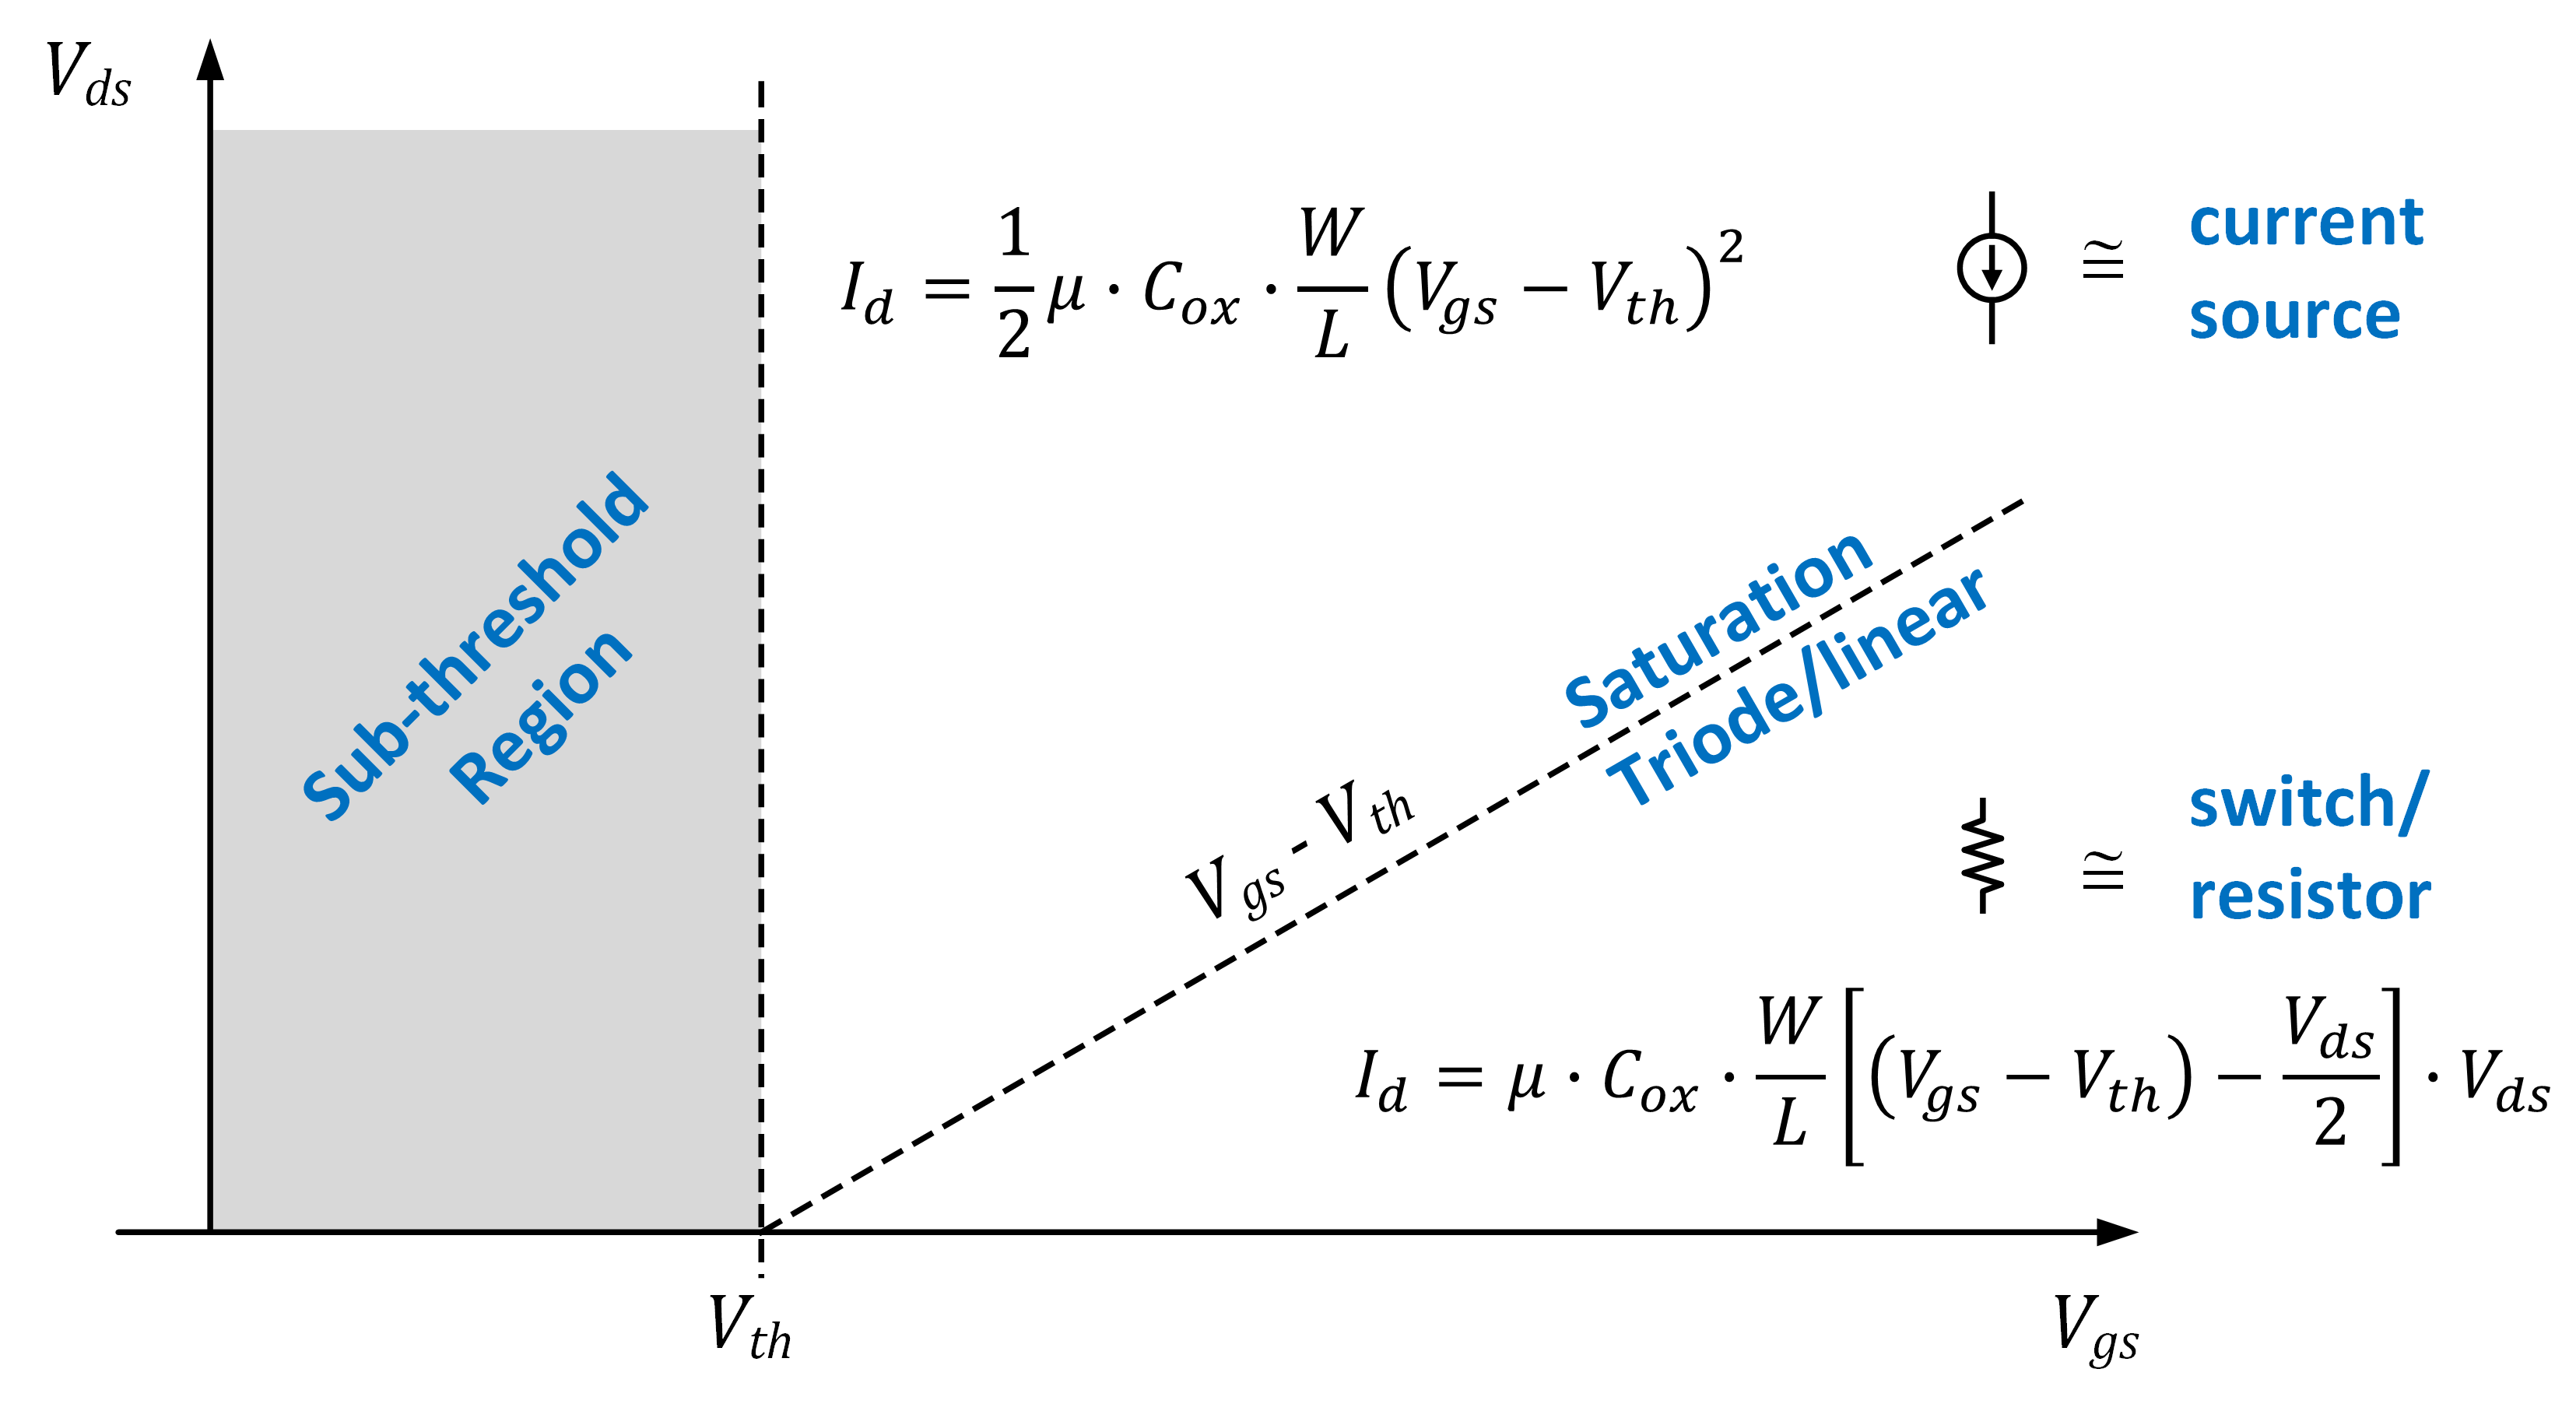
\includegraphics{MOS_regions_summary.png}
\caption{MOS\_regions\_summary.png}
\end{figure}

    \hypertarget{dc-small-signal-model}{%
\subsection{DC small-signal model}\label{dc-small-signal-model}}

    \begin{figure}
\centering
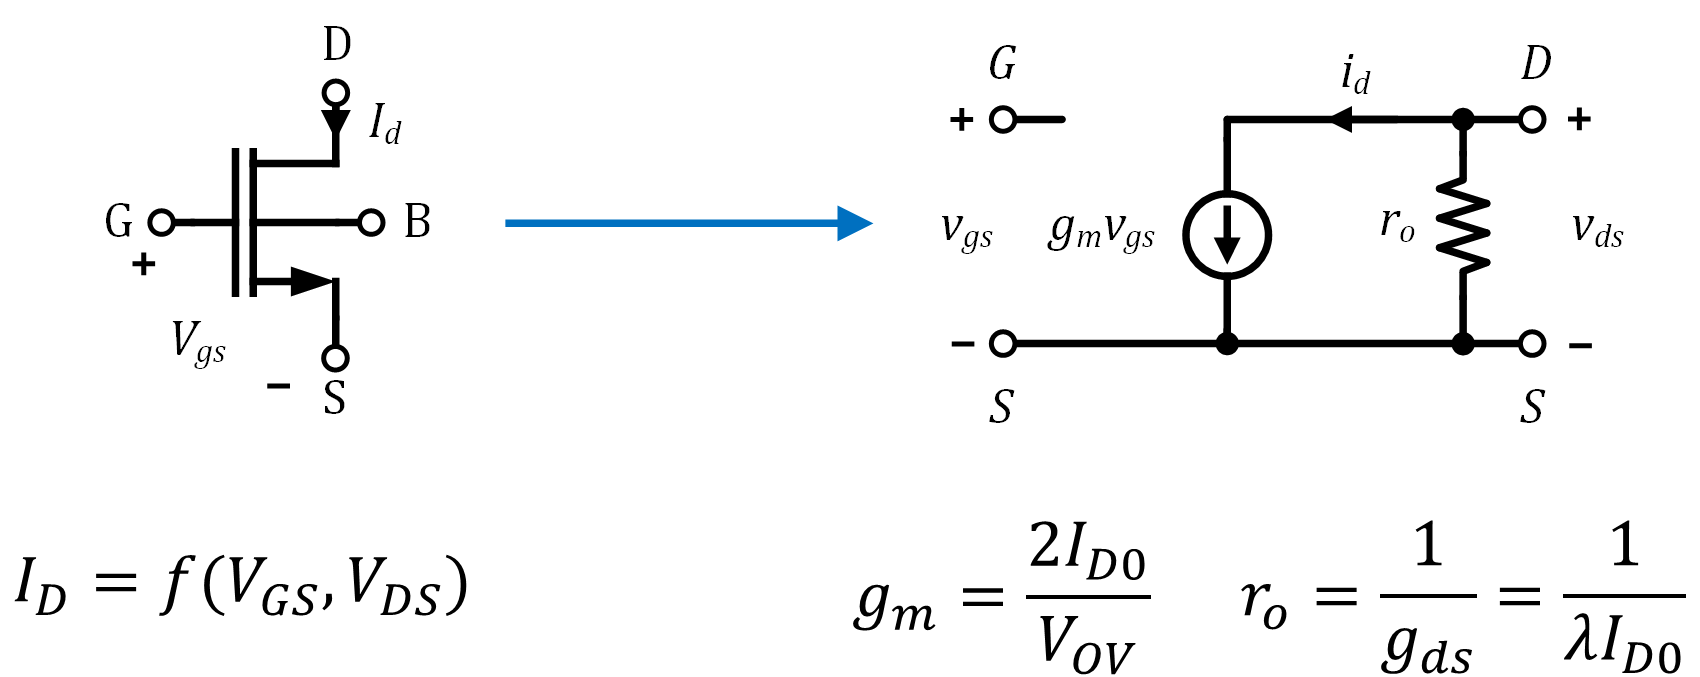
\includegraphics{DC_small_signal_model.png}
\caption{DC\_small\_signal\_model.png}
\end{figure}

    \begin{itemize}
\tightlist
\item
  Small-signal model replaces nonlinear \(I_D(V_{GS}, V_{DS})\) with
  linear parameters \(g_m\) and \(r_o\) that enable the use of linear
  circuit analysis techniques
\item
  \emph{Important}: All DC voltages become AC ground in the small-signal
  model
\end{itemize}

    \hypertarget{pmos-transistor}{%
\subsection{PMOS transistor}\label{pmos-transistor}}

    \begin{figure}
\centering
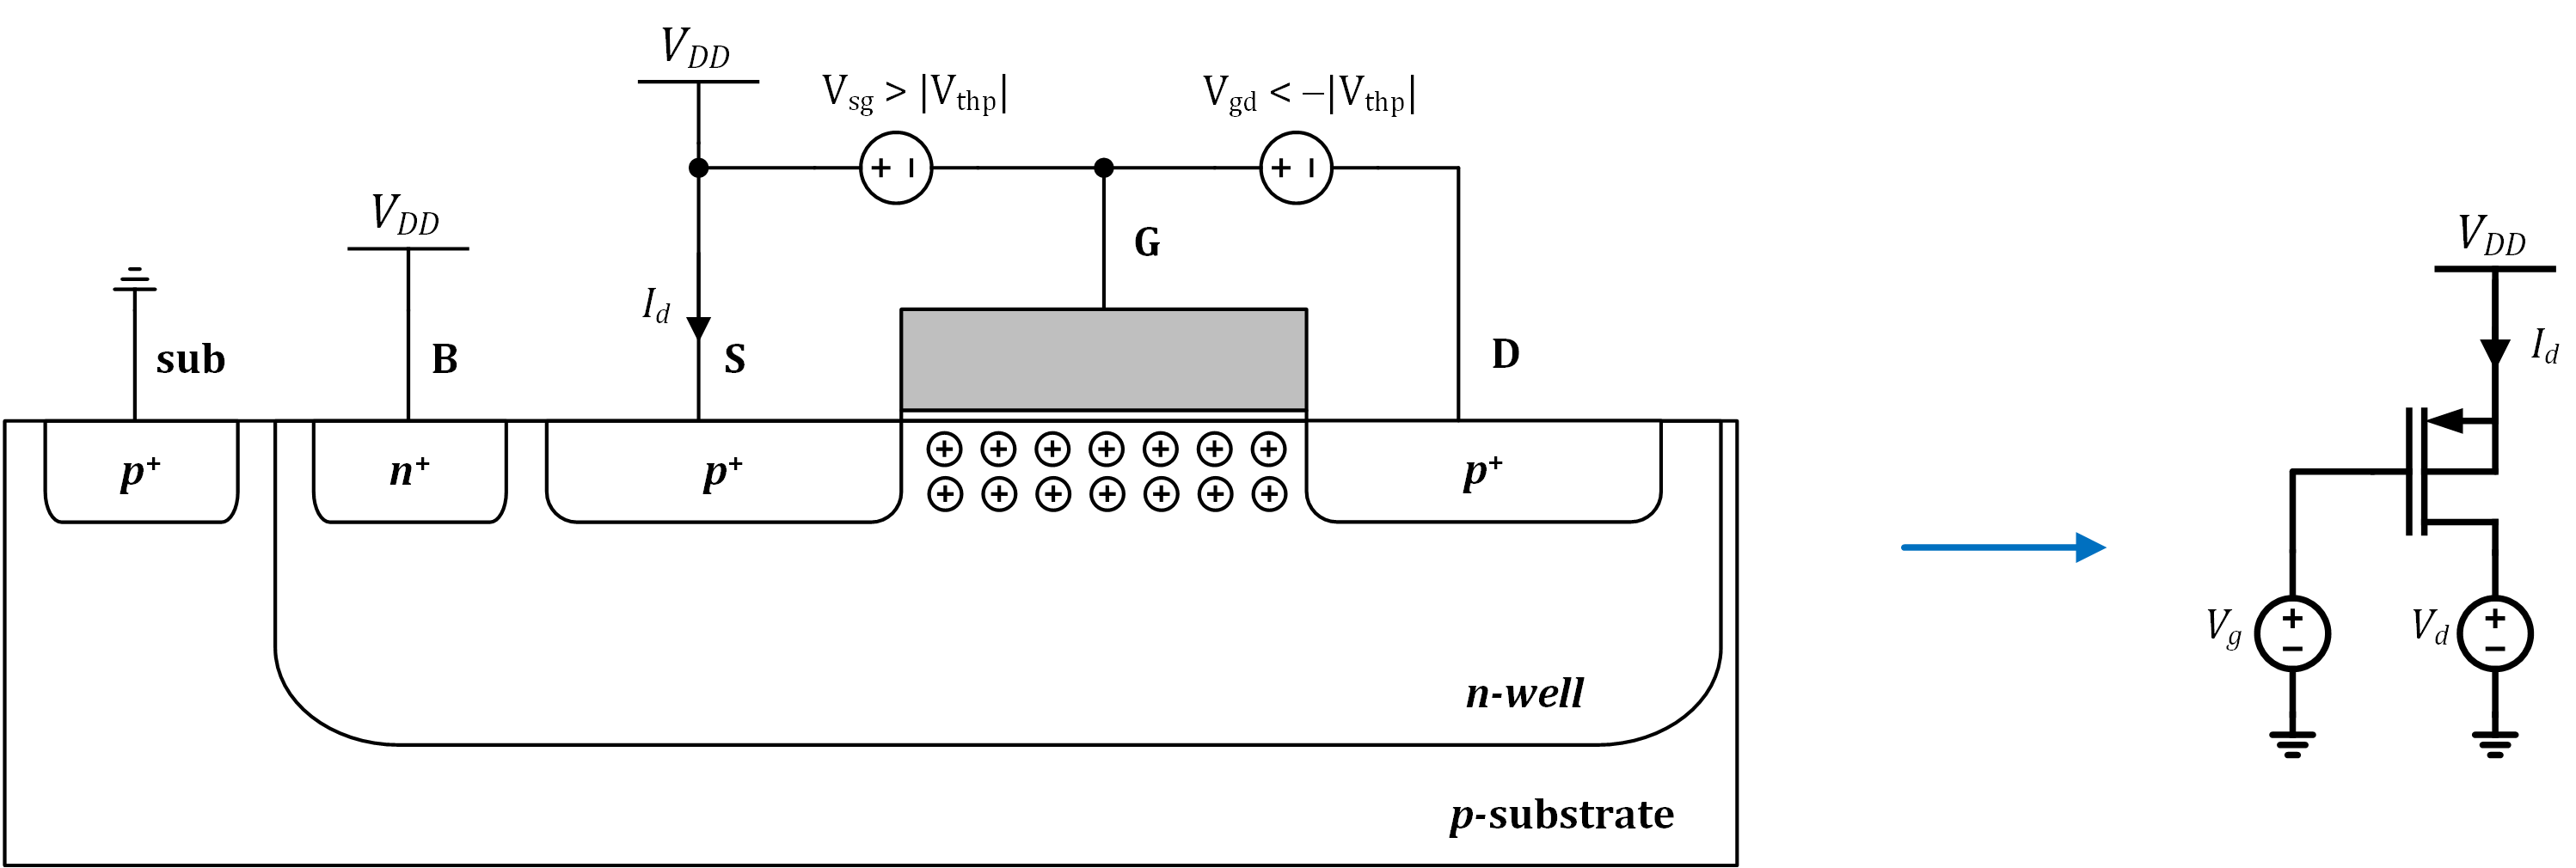
\includegraphics{PMOS_saturation.png}
\caption{PMOS\_saturation.png}
\end{figure}

    \begin{itemize}
\tightlist
\item
  In \(CMOS\) processes, \(PMOS\) transistors are produced in the same
  substrate as NMOS
\item
  To operate in saturation, the following requirements must be
  satisfied:

  \begin{itemize}
  \tightlist
  \item
    \(V_{sg} > |V_{thp}|\)
  \item
    \(V_{sd} > V_{sg} - |V_{thp}|\)
  \end{itemize}
\item
  The saturation current for a \(PMOS\) transistor is thus given by
\end{itemize}

\begin{equation}
I_d = \dfrac{1}{2}\mu_p C_{ox} \dfrac{W}{L} (V_{sg} - |V_{thp}|)^2(1+\lambda V_{sd})
\end{equation}

    \hypertarget{high-gain-amplifier-design}{%
\subsection{High-gain amplifier
design}\label{high-gain-amplifier-design}}

    \begin{figure}
\centering
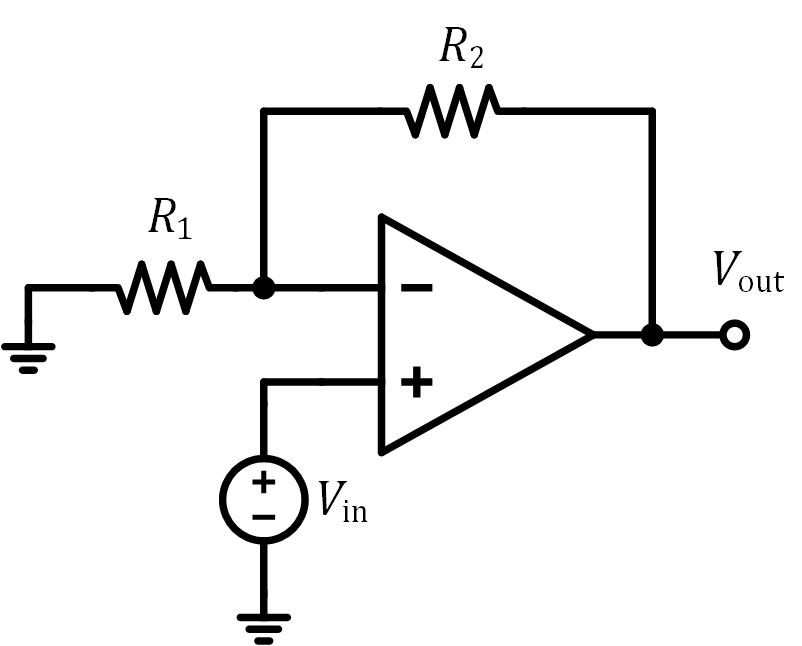
\includegraphics{non_inverting_amplifier.png}
\caption{non\_inverting\_amplifier.png}
\end{figure}

    \begin{align}
G &= \dfrac{V_{out}}{V_{in}} = \dfrac{A_v}{1+\beta A_v}
\end{align}

\begin{equation}
\beta = \dfrac{R_1}{R_1+R_2}
\end{equation}

\begin{itemize}
\tightlist
\item
  if \(\beta A_v\) \(>> 1\),
\end{itemize}

\begin{equation}
G = \dfrac{A_v}{1+\beta A_v} \rightarrow \dfrac{1}{\beta}
\end{equation}

    \begin{itemize}
\tightlist
\item
  High-gain amplifiers are used to desensitize transfer functions to
  temperature- and manufacturing-dependent physical parameters
  (e.g.~\(g_m\) and \(r_o\))
\item
  Typical values of \(A_v\) for opamps are \(100 - 140 dB\)
  (\(100,000 - 10,000,000 V/V\))
\item
  High \emph{open-loop} gain (\(A_v\)) \(\rightarrow\) precise
  \emph{closed-loop} gain (\(G\))
\item
  For this reason, when designing CMOS amplifiers (i.e.~opamps and OTAs)
  substantial emphasis is placed on achieving high open-loop gain
\end{itemize}

    \hypertarget{common-source-amplifier}{%
\subsection{Common-source amplifier}\label{common-source-amplifier}}

    \begin{figure}
\centering
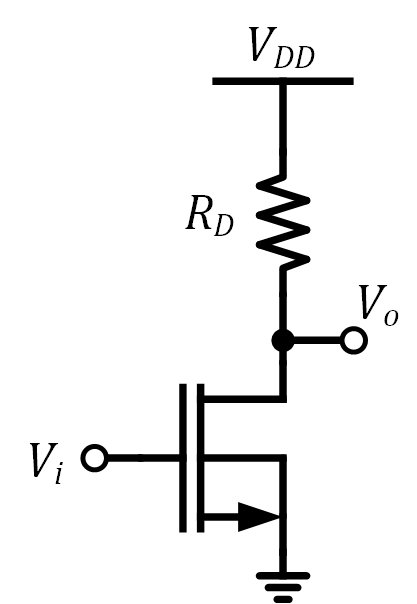
\includegraphics{common_source_amplifier.png}
\caption{common\_source\_amplifier.png}
\end{figure}

    \begin{equation}
I_d = \dfrac{1}{2}\mu\cdot C_{ox} \cdot \dfrac{W}{L}(V_{i}-V_{th})^2 (1+\lambda V_{o})
\end{equation}

\begin{equation}
V_o = V_{DD} - I_d\cdot R_D
\end{equation}

    \begin{itemize}
\tightlist
\item
  The common-source amplifier is an exemplary model of how we achieve
  gain in analog circuits:

  \begin{itemize}
  \tightlist
  \item
    Change in the output current \(\Delta I_d\) is realized (primarily)
    by a change in the input voltage \(\Delta V_i\) and the
    voltage-current relationship of the device
  \item
    Output voltage changes as the result of \(\Delta I_d\) flowing
    through the output resistance of the circuit (in this case, \(R_D\))
  \end{itemize}
\end{itemize}

    \hypertarget{ouput-voltage-minimummaximum-swing}{%
\subsection{Ouput voltage minimum/maximum
(swing)}\label{ouput-voltage-minimummaximum-swing}}

    \begin{itemize}
\tightlist
\item
  For the maximum voltage, when \(V_o = V_{DD}\), current no longer
  flows through \(R_D\) and changes in the input cannot effect changes
  in the output
\item
  For the minimum, to ensure the transistor remains in saturation
  \(V_o\) should be greater than the overdrive voltage, \(V_i - V_{th}\)
\item
  The valid range of output voltages is thus
\end{itemize}

\begin{equation}
V_i - V_{th} < V_o < V_{DD}
\end{equation}

\begin{itemize}
\tightlist
\item
  Assuming signals swing symmetrically above and below the operating
  point, we can maximize use of the output swing by selecting \(R_D\)
  and \(I_D\) to an output operating point at the output of
  \(V_O = V_{DD}/2\)
\end{itemize}

    \hypertarget{small-signal-model}{%
\subsection{Small-signal model}\label{small-signal-model}}

    \begin{figure}
\centering
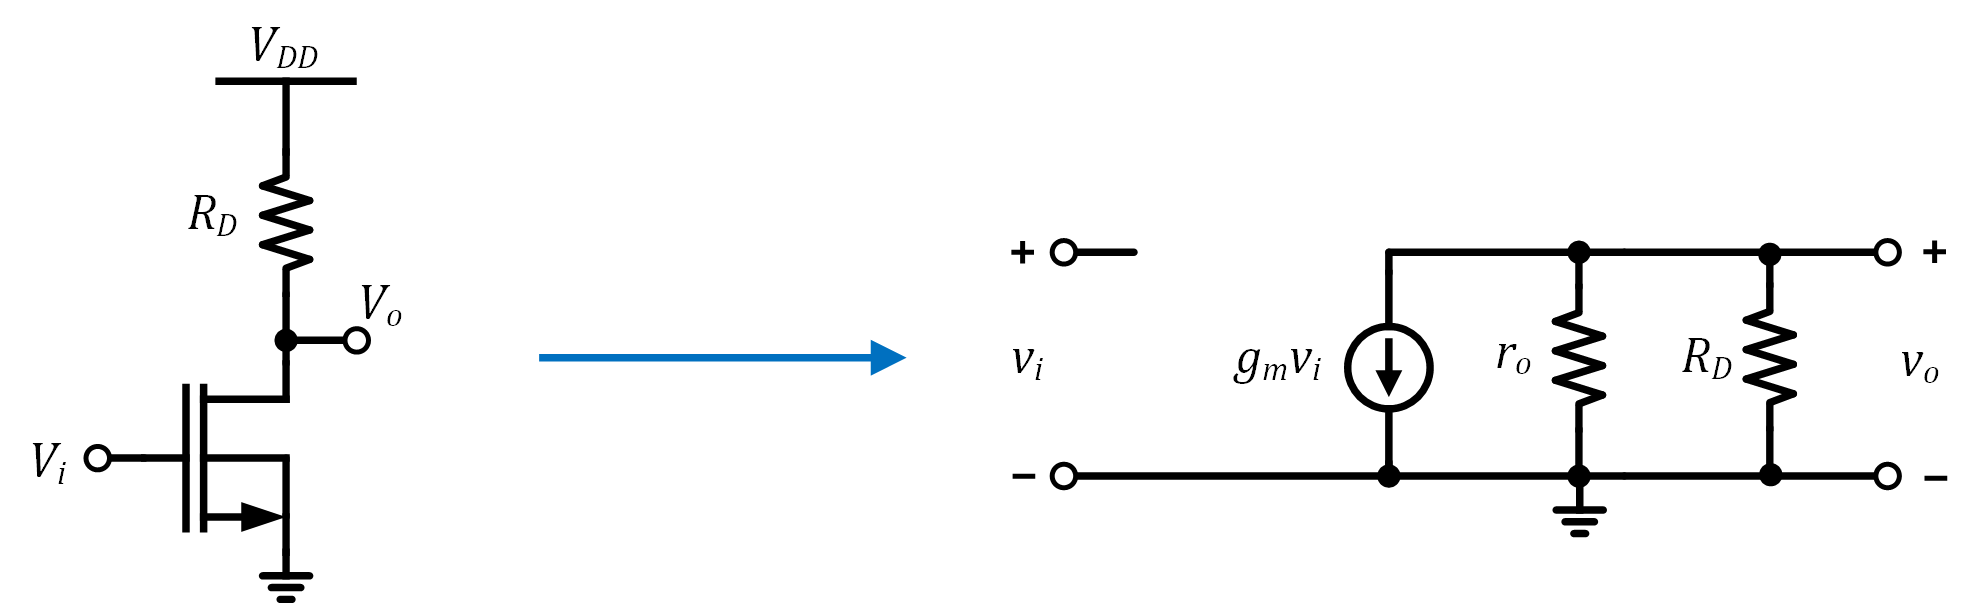
\includegraphics{common_source_small_signal.png}
\caption{common\_source\_small\_signal.png}
\end{figure}

    \begin{itemize}
\tightlist
\item
  \(V_{DD}\) is a \(DC\) (constant) voltage, making it an \(AC\)
  (small-signal) ground
\item
  \(r_o\) and \(R_D\) appear in parallel in the small-signal model
\end{itemize}

    \hypertarget{mos-amplifier-analysis}{%
\subsection{MOS amplifier analysis}\label{mos-amplifier-analysis}}

    \begin{figure}
\centering
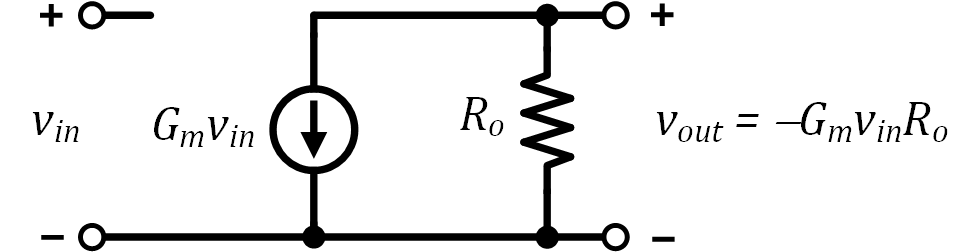
\includegraphics{norton_amplifier_model.png}
\caption{norton\_amplifier\_model.png}
\end{figure}

    \begin{itemize}
\tightlist
\item
  Voltage gain in transistor-based circuits is \emph{almost always}
  realized as the product of a transconductance \(G_m\) and a
  small-signal resistance \(R_o\)
\item
  Analysis approach: Use Norton analysis to determine the parameters
  \(G_m\) and \(R_o\) using the small signal model

  \begin{itemize}
  \tightlist
  \item
    Find the short-circuit current \(i_{sc}\) to determine
    \(G_m = i_{sc}/v_{in}\)
  \item
    The output resistance \(R_o\) is determiend by setting
    \(v_{in} = 0\), applying a test voltage to the output, and finding
    the expression for the resulting current
  \end{itemize}
\end{itemize}

    \hypertarget{common-source-norton-model-gm}{%
\subsection{Common-source Norton model
(Gm)}\label{common-source-norton-model-gm}}

    \begin{figure}
\centering
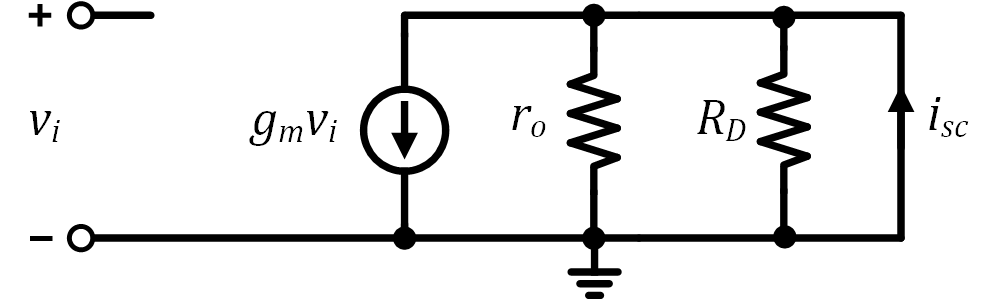
\includegraphics{common_source_Gm.png}
\caption{common\_source\_Gm.png}
\end{figure}

    \begin{itemize}
\tightlist
\item
  To determine \(G_m\) in the Norton model, short the output terminals
  and measure \(i_{sc}\)
\item
  Due to the short circuit, no current flows through \(r_o\) or \(R_D\)
\item
  \(G_m\) is determined by taking the ratio of \(i_{sc}\) to \(v_i\):
\end{itemize}

\begin{equation}
G_m = \dfrac{i_{sc}}{v_i} = \dfrac{g_m \cdot v_i}{v_i}= g_m
\end{equation}

\begin{itemize}
\tightlist
\item
  Thus, in the case of the common-source amplifier, \(G_m = g_m\)
\end{itemize}

    \hypertarget{common-source-norton-model-ro}{%
\subsection{Common-source Norton model
(Ro)}\label{common-source-norton-model-ro}}

    \begin{figure}
\centering
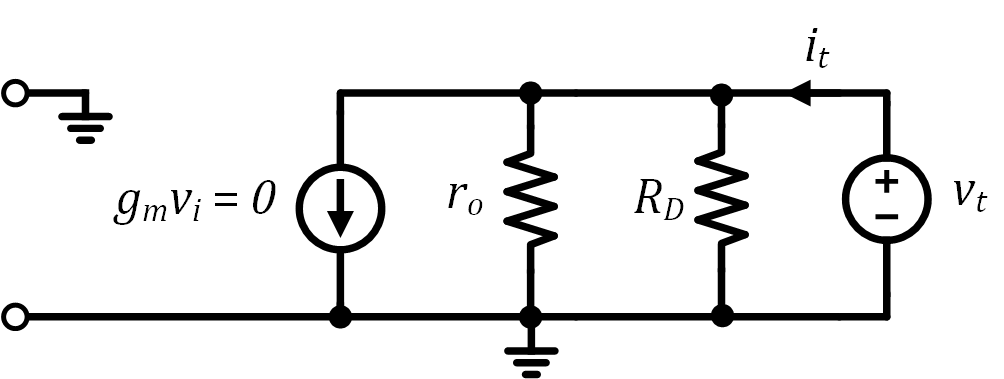
\includegraphics{common_source_Ro.png}
\caption{common\_source\_Ro.png}
\end{figure}

    \begin{itemize}
\tightlist
\item
  To determine \(R_o\), apply a test voltage \(v_t\) between the output
  terminals and measure \(i_t\)
\item
  Here we can see that \(i_t\) is given by
\end{itemize}

\begin{equation}
i_t = v_t \cdot \left(\dfrac{1}{r_o} + \dfrac{1}{R_D} \right)
\end{equation}

\begin{itemize}
\tightlist
\item
  Thus, \(R_o\) is just the parallel combination of \(r_o\) and \(R_D\):
\end{itemize}

\begin{equation}
R_o = \dfrac{v_t}{i_t} = \left(\dfrac{1}{r_o}+ \dfrac{1}{R_D} \right)^{-1} = \boxed{r_o || R_D}
\end{equation}

\begin{itemize}
\tightlist
\item
  The voltage gain is thus
\end{itemize}

\begin{equation}
-G_m \cdot R_o = -g_m \cdot r_o || R_D
\end{equation}

    \hypertarget{relative-magnitudes-of-rd-and-ro}{%
\subsection{Relative magnitudes of RD and
ro}\label{relative-magnitudes-of-rd-and-ro}}

    \begin{itemize}
\tightlist
\item
  Output resistance \(r_o\) is given by the expression
\end{itemize}

\begin{equation}
r_o \approx \dfrac{1}{\lambda I_{D0}}
\end{equation}

\begin{itemize}
\tightlist
\item
  Typical drain resistance \(R_D\) can be expressed as (assumes output
  DC operating point of \(V_{DD}/2\), which allows for maximal output
  signal swing)
\end{itemize}

\begin{equation}
R_D \approx \dfrac{V_{DD}}{2I_{D0}}
\end{equation}

\begin{itemize}
\tightlist
\item
  For \(V_{DD} = 3V\) and \(\lambda = 0.1V^{-1}\),
  \(r_o \approx 7 \times R_D\)
\item
  Thus, for the common-source amplifier,
\end{itemize}

\begin{equation}
\boxed{A_v = -g_m(r_o||R_D) \approx -g_m\cdot R_D}
\end{equation}

    \hypertarget{maximum-gain-with-rd}{%
\subsection{Maximum gain with RD}\label{maximum-gain-with-rd}}

    \begin{itemize}
\tightlist
\item
  What is the maximum gain that can be achieved with a passive
  (resistive) load?
\end{itemize}

\begin{equation}
A_v \approx -g_m\cdot R_D = -\dfrac{2I_{D0}}{V_{ov}}R_D
\end{equation}

\begin{itemize}
\tightlist
\item
  Assuming an operating point for the output voltage of \(V_{DD}/2\),
  the gain is given by
\end{itemize}

\begin{equation}
|A_v| \approx \dfrac{2\cdot V_{DD}/2}{R_D\cdot V_{ov}}\cdot R_D = \dfrac{V_{DD}}{V_{ov}}
\end{equation}

\begin{itemize}
\tightlist
\item
  Assuming \(V_{DD} = 3V\) and \(V_{ov} = 150mV\), this limits the gain
  to approximately \(20V/V\)
\item
  This is generally too low to be useful in building an opamp
\item
  How do we increase gain?
\end{itemize}

    \hypertarget{mos-dc-model-intrinsic-gain}{%
\subsection{MOS DC model (intrinsic
gain)}\label{mos-dc-model-intrinsic-gain}}

    \begin{figure}
\centering
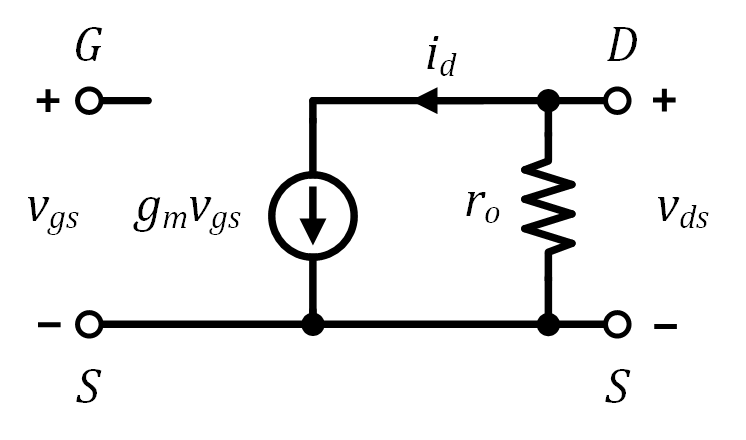
\includegraphics{MOS_intrinsic_gain.png}
\caption{MOS\_intrinsic\_gain.png}
\end{figure}

    \begin{equation}
g_m = \dfrac{2I_{D0}}{V_{OV}}
\end{equation}

\begin{equation}
r_o = \dfrac{1}{g_{ds}} = \dfrac{1}{\lambda I_{D0}}
\end{equation}

\begin{equation}
\left|\dfrac{v_{ds}}{v_{gs}}\right| = \dfrac{g_m}{g_{ds}} = \dfrac{2}{\lambda V_{OV}}
\end{equation}

    \begin{itemize}
\tightlist
\item
  Recall that the intrisic gain of the transistor is given by the
  product of \(g_m\) and \(r_o\)
\item
  \(g_m\) increases linearly with drain current, while \(r_o\) is
  inversely dependent, keeping their product constant
\item
  What is a typical value for \(g_m r_o\)?
\end{itemize}

    \hypertarget{intrinsic-gain}{%
\subsection{Intrinsic gain}\label{intrinsic-gain}}

    \begin{itemize}
\tightlist
\item
  In our Level 1 ``process'' \(\lambda_n = 0.1 V^{-1}\)
\item
  In order to maximize signal swing, we want to use a relatively low
  overdrive voltage (\(V_{ov} = V_{GS} - V_{th}\))
\item
  Assuming a gate bias of \(V_{GS0} = 0.9V\) (for example), the
  intrinsic gain is given as
\end{itemize}

\begin{equation}
g_mr_o \approx \dfrac{2}{\lambda V_{ov}} = \dfrac{2}{0.1 V^{-1} \times 200mV} = 100 V/V
\end{equation}

\begin{itemize}
\tightlist
\item
  This is \(5 \times\) the theoretical gain with a resistive load
\item
  How can we can advantage of intrinsic gain to build amplifiers with
  gains approaching/exceeding \(100dB\)?
\end{itemize}

    \hypertarget{common-source-with-active-load}{%
\subsection{Common-source with active
load}\label{common-source-with-active-load}}

    \begin{figure}
\centering
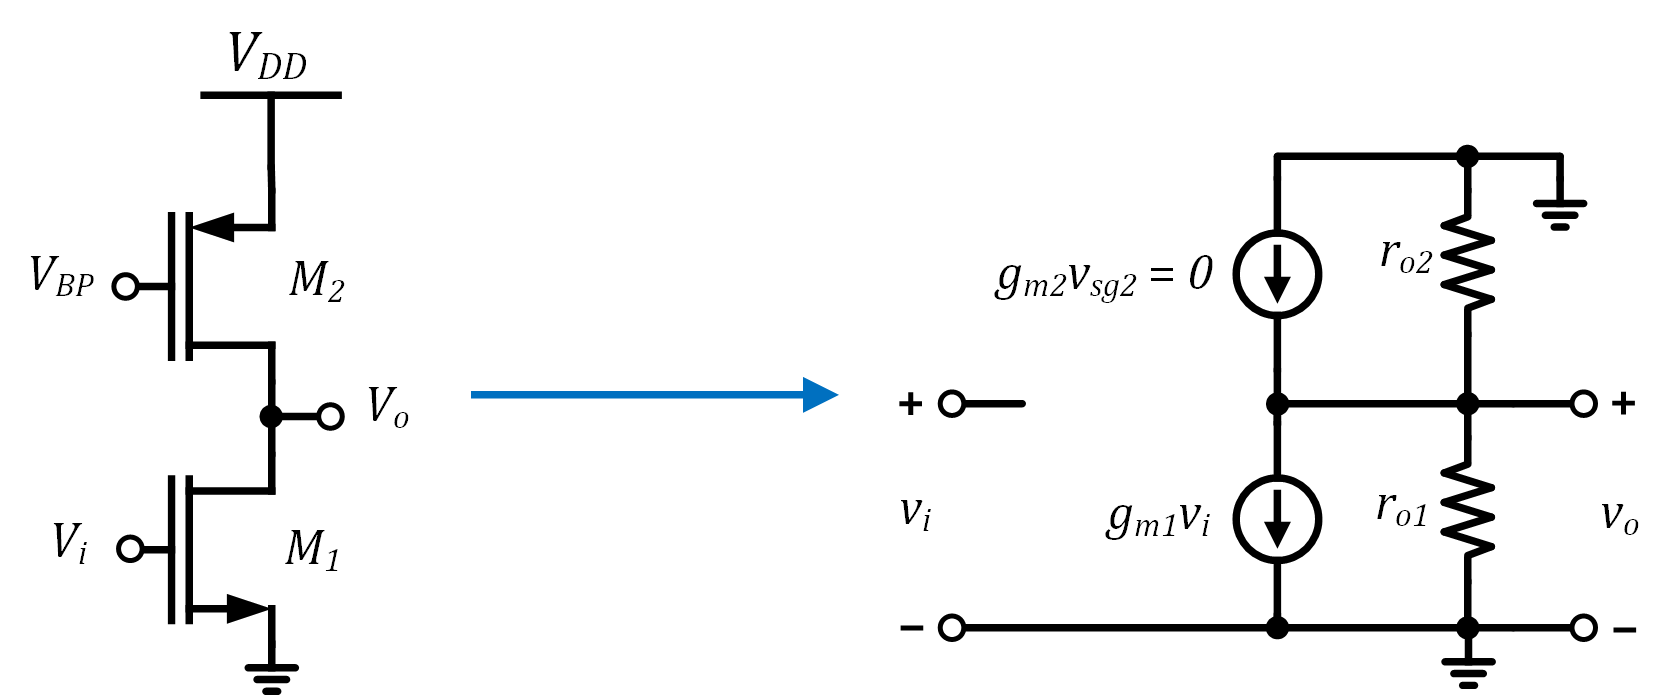
\includegraphics{common_source_active_small_signal.png}
\caption{common\_source\_active\_small\_signal.png}
\end{figure}

    \begin{itemize}
\tightlist
\item
  We can increase the gain of the common-source statge by replacing the
  resistor \(R_D\)with a \(PMOS\) transistor in saturation
\item
  This is referred to as an \emph{active} load, since it replaces a
  passive device (resistor) with an active one (transistor)
\item
  The bias voltage \(V_{BP}\) sets the \(DC\) operating point
  (\(g_{m1,2}\) and \(r_{o1,2}\)) of the amplifier stage by controlling
  the drain currents of \(M_1\) and \(M_2\)
\item
  Because both \(V_S\) and \(V_G\) of \(M_2\) are \(DC\) voltages, its
  transconductance current is zero in the small-signal model
\end{itemize}

    \hypertarget{small-signal-gain}{%
\subsection{Small-signal gain}\label{small-signal-gain}}

    \begin{figure}
\centering
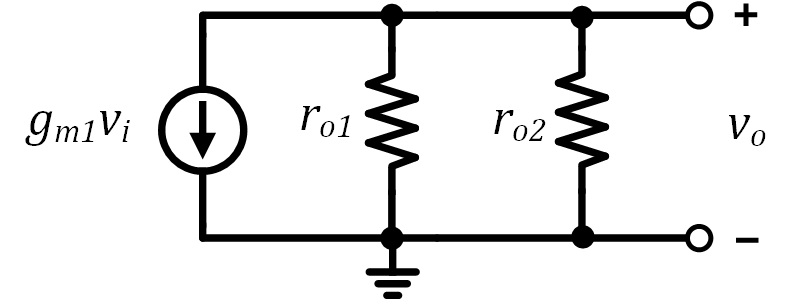
\includegraphics{CS_active_small_signal.png}
\caption{CS\_active\_small\_signal.png}
\end{figure}

    \begin{itemize}
\tightlist
\item
  In this circuit, \(M_1\) functions as a transconductor and \(M_2\)
  behaves as a resistance
\item
  The small-signal gain expression is identical to that of the passive
  load, with \(R_D\) replaced by \(r_{o2}\):
\end{itemize}

\begin{equation}
A_v = \dfrac{v_o}{v_i} = -g_{m1} \cdot (r_{o1} || r_{o2})
\end{equation}

\begin{itemize}
\tightlist
\item
  If we make the (somewhat dubious) assumption that
  \(r_{op} = r_{on} = r_o\), we can relate the gain of the active load
  stage to the MOSFET's intrinsic gain:
\end{itemize}

\begin{equation}
A_v = \dfrac{v_o}{v_i} = -g_{m1} \cdot (r_{o1} || r_{o2}) \approx -\dfrac{g_m\cdot r_o}{2}
\end{equation}

\begin{itemize}
\tightlist
\item
  In practice \(r_{on} \neq r_{op}\), but are of the same order of
  magnitude
\end{itemize}

    \hypertarget{magnitude-of-the-gain}{%
\subsection{Magnitude of the gain}\label{magnitude-of-the-gain}}

    \begin{itemize}
\tightlist
\item
  Recall that the gain of the common-source stage with a passive load
  (\(R_D\)) is
\end{itemize}

\begin{equation}
A_v = -g_m(r_o||R_D) \approx -g_m\cdot R_D
\end{equation}

\begin{itemize}
\tightlist
\item
  For a nominal \(DC\) output votage of \(V_{DD}/2\) (i.e.~the \(DC\)
  operating point), this is
\end{itemize}

\begin{equation}
|A_v| \approx \dfrac{2\cdot V_{DD}/2}{R_D\cdot V_{ov}}\cdot R_D = \dfrac{V_{DD}}{V_{ov}} \leq 20V/V
\end{equation}

\begin{itemize}
\tightlist
\item
  For the active-load stage, the gain is given by
\end{itemize}

\begin{equation}
A_v = \dfrac{v_o}{v_i} = -g_{m1} \cdot (r_{o1} || r_{o2})
\end{equation}

\begin{itemize}
\tightlist
\item
  Using our Level 1 process parameters
  (\(\lambda_n = 0.1, \lambda_p = 0.2\)), this becomes
\end{itemize}

\begin{equation}
A_v = -g_{m1} \cdot (r_{o1} || r_{o2}) = -g_{m1}\cdot r_{o1} \dfrac{r_{o2}}{r_{o1} + r_{o2}}\approx -33 V/V
\end{equation}

\begin{itemize}
\tightlist
\item
  This is an improvement, but still fairly low. We'll discuss how to
  increase this soon\ldots{}
\end{itemize}

    \hypertarget{ouput-voltage-range}{%
\subsection{Ouput voltage range}\label{ouput-voltage-range}}

    \begin{itemize}
\tightlist
\item
  When \(V_o\) is at its maximum value, \(M_2\) still needs to be in
  saturation to operate as a high-resistance load, requiring
\end{itemize}

\begin{equation}
V_o < V_{DD} - (V_{DD}  - V_{BP} + |V_{thp}|) = V_{BP} - |V_{thp}|
\end{equation}

\begin{itemize}
\tightlist
\item
  Similarly, \(M_1\) needs to remain in saturation, setting the lower
  bound on \(V_o\) as
\end{itemize}

\begin{equation}
V_o > V_{GS1} - V_{thn}
\end{equation}

\begin{itemize}
\tightlist
\item
  The valid range of output voltages is thus
\end{itemize}

\begin{equation}
V_{GS1} - V_{thn} < V_o < V_{BP} - |V_{thp}|
\end{equation}

\begin{itemize}
\tightlist
\item
  One way to look at this is to say the output swing is
  \(V_{DD} - 2V_{OV}\)
\item
  Again to maximize use of this range we would like to set the operating
  point of \(V_o\) to approximately \(V_{DD}/2\)
\item
  How do we set the operating point?
\end{itemize}

    \begin{tcolorbox}[breakable, size=fbox, boxrule=1pt, pad at break*=1mm,colback=cellbackground, colframe=cellborder]
\prompt{In}{incolor}{3}{\boxspacing}
\begin{Verbatim}[commandchars=\\\{\}]
\PY{k}{def} \PY{n+nf}{plot\PYZus{}cs\PYZus{}op\PYZus{}point}\PY{p}{(}\PY{n}{V\PYZus{}DD}\PY{p}{,} \PY{n}{V\PYZus{}BP}\PY{p}{,} \PY{n}{V\PYZus{}GS1}\PY{p}{,} \PY{n}{V\PYZus{}out}\PY{p}{)}\PY{p}{:}
    \PY{n}{I\PYZus{}d1} \PY{o}{=} \PY{n}{nmos\PYZus{}iv\PYZus{}sweep}\PY{p}{(}\PY{n}{V\PYZus{}GS1}\PY{p}{,} \PY{n}{V\PYZus{}out}\PY{p}{,} \PY{l+m+mi}{100}\PY{p}{,} \PY{l+m+mi}{1}\PY{p}{,} \PY{l+m+mf}{0.1}\PY{p}{)}
    \PY{n}{I\PYZus{}d2} \PY{o}{=} \PY{n}{pmos\PYZus{}iv\PYZus{}sweep}\PY{p}{(}\PY{n}{V\PYZus{}DD}\PY{o}{\PYZhy{}}\PY{n}{V\PYZus{}BP}\PY{p}{,} \PY{n}{V\PYZus{}DD}\PY{o}{\PYZhy{}}\PY{n}{V\PYZus{}out}\PY{p}{,} \PY{l+m+mi}{200}\PY{p}{,} \PY{l+m+mi}{1}\PY{p}{,} \PY{l+m+mf}{0.2}\PY{p}{)}
    
    \PY{n}{fig}\PY{p}{,} \PY{n}{ax} \PY{o}{=} \PY{n}{plt}\PY{o}{.}\PY{n}{subplots}\PY{p}{(}\PY{n}{figsize}\PY{o}{=}\PY{p}{(}\PY{l+m+mf}{10.0}\PY{p}{,} \PY{l+m+mf}{7.5}\PY{p}{)}\PY{p}{)}
    \PY{n}{ax}\PY{o}{.}\PY{n}{plot}\PY{p}{(}\PY{n}{V\PYZus{}out}\PY{p}{,} \PY{l+m+mf}{1e6}\PY{o}{*}\PY{n}{I\PYZus{}d1}\PY{p}{,} \PY{n}{label}\PY{o}{=}\PY{l+s+sa}{r}\PY{l+s+s1}{\PYZsq{}}\PY{l+s+s1}{\PYZdl{}I\PYZus{}}\PY{l+s+s1}{\PYZob{}}\PY{l+s+s1}{d,NMOS\PYZcb{}\PYZdl{}}\PY{l+s+s1}{\PYZsq{}}\PY{p}{,} \PY{n}{color}\PY{o}{=}\PY{l+s+s1}{\PYZsq{}}\PY{l+s+s1}{blue}\PY{l+s+s1}{\PYZsq{}}\PY{p}{)}
    \PY{n}{ax}\PY{o}{.}\PY{n}{plot}\PY{p}{(}\PY{n}{V\PYZus{}out}\PY{p}{,} \PY{l+m+mf}{1e6}\PY{o}{*}\PY{n}{I\PYZus{}d2}\PY{p}{,} \PY{n}{label}\PY{o}{=}\PY{l+s+sa}{r}\PY{l+s+s1}{\PYZsq{}}\PY{l+s+s1}{\PYZdl{}I\PYZus{}}\PY{l+s+s1}{\PYZob{}}\PY{l+s+s1}{d,PMOS\PYZcb{}\PYZdl{}}\PY{l+s+s1}{\PYZsq{}}\PY{p}{,} \PY{n}{color}\PY{o}{=}\PY{l+s+s1}{\PYZsq{}}\PY{l+s+s1}{red}\PY{l+s+s1}{\PYZsq{}}\PY{p}{)}
    \PY{n}{ax}\PY{o}{.}\PY{n}{set\PYZus{}xlabel}\PY{p}{(}\PY{l+s+sa}{r}\PY{l+s+s1}{\PYZsq{}}\PY{l+s+s1}{\PYZdl{}V\PYZus{}}\PY{l+s+si}{\PYZob{}out\PYZcb{}}\PY{l+s+s1}{ [V]\PYZdl{}}\PY{l+s+s1}{\PYZsq{}}\PY{p}{)}
    \PY{n}{ax}\PY{o}{.}\PY{n}{set\PYZus{}ylabel}\PY{p}{(}\PY{l+s+sa}{r}\PY{l+s+s1}{\PYZsq{}}\PY{l+s+s1}{\PYZdl{}I\PYZus{}}\PY{l+s+si}{\PYZob{}d\PYZcb{}}\PY{l+s+s1}{ [}\PY{l+s+s1}{\PYZbs{}}\PY{l+s+s1}{mu A]\PYZdl{}}\PY{l+s+s1}{\PYZsq{}}\PY{p}{)}
    \PY{n}{ax}\PY{o}{.}\PY{n}{legend}\PY{p}{(}\PY{p}{)}
    \PY{n}{ax}\PY{o}{.}\PY{n}{grid}\PY{p}{(}\PY{p}{)}
\end{Verbatim}
\end{tcolorbox}

    \begin{itemize}
\tightlist
\item
  Because \(I_{D1} = I_{D2}\), the point at which the drain current
  curves intersect constitutes the operating point of the circuit
\item
  For a nominal (\(DC\)) input voltage of \(0.86V\), both transistors
  are approximately in the middle of their saturation ranges and the
  output voltage is \textasciitilde{}\(V_{DD}/2\)
\item
  However, if \(V_{GS1}\) is changed slightly (or if device parameters
  differ due to manufacturing variability), the resulting operating
  point can place either \(M_1\) or \(M_2\) in triode, drastically
  decreasing the gain
\item
  Feedback is required to stabilize the output DC voltage at a desired
  value (more on this later)
\end{itemize}

    \begin{tcolorbox}[breakable, size=fbox, boxrule=1pt, pad at break*=1mm,colback=cellbackground, colframe=cellborder]
\prompt{In}{incolor}{6}{\boxspacing}
\begin{Verbatim}[commandchars=\\\{\}]
\PY{n}{V\PYZus{}DD} \PY{o}{=} \PY{l+m+mi}{3}
\PY{n}{V\PYZus{}BP} \PY{o}{=} \PY{l+m+mi}{2}
\PY{n}{V\PYZus{}GS1} \PY{o}{=} \PY{o}{.}\PY{l+m+mi}{86} 
\PY{n}{V\PYZus{}out} \PY{o}{=} \PY{n}{np}\PY{o}{.}\PY{n}{arange}\PY{p}{(}\PY{l+m+mi}{0}\PY{p}{,}\PY{l+m+mi}{3}\PY{p}{,}\PY{n}{step}\PY{o}{=}\PY{l+m+mf}{0.01}\PY{p}{)}
\PY{n}{plot\PYZus{}cs\PYZus{}op\PYZus{}point}\PY{p}{(}\PY{n}{V\PYZus{}DD}\PY{p}{,} \PY{n}{V\PYZus{}BP}\PY{p}{,} \PY{n}{V\PYZus{}GS1}\PY{p}{,} \PY{n}{V\PYZus{}out}\PY{p}{)}
\end{Verbatim}
\end{tcolorbox}

    \begin{center}
    \adjustimage{max size={0.9\linewidth}{0.9\paperheight}}{2021_01_13_EE538_Lecture2_W2021_files/2021_01_13_EE538_Lecture2_W2021_62_0.png}
    \end{center}
    { \hspace*{\fill} \\}
    
    \hypertarget{common-source-biasing}{%
\subsection{Common-source biasing}\label{common-source-biasing}}

    \begin{figure}
\centering
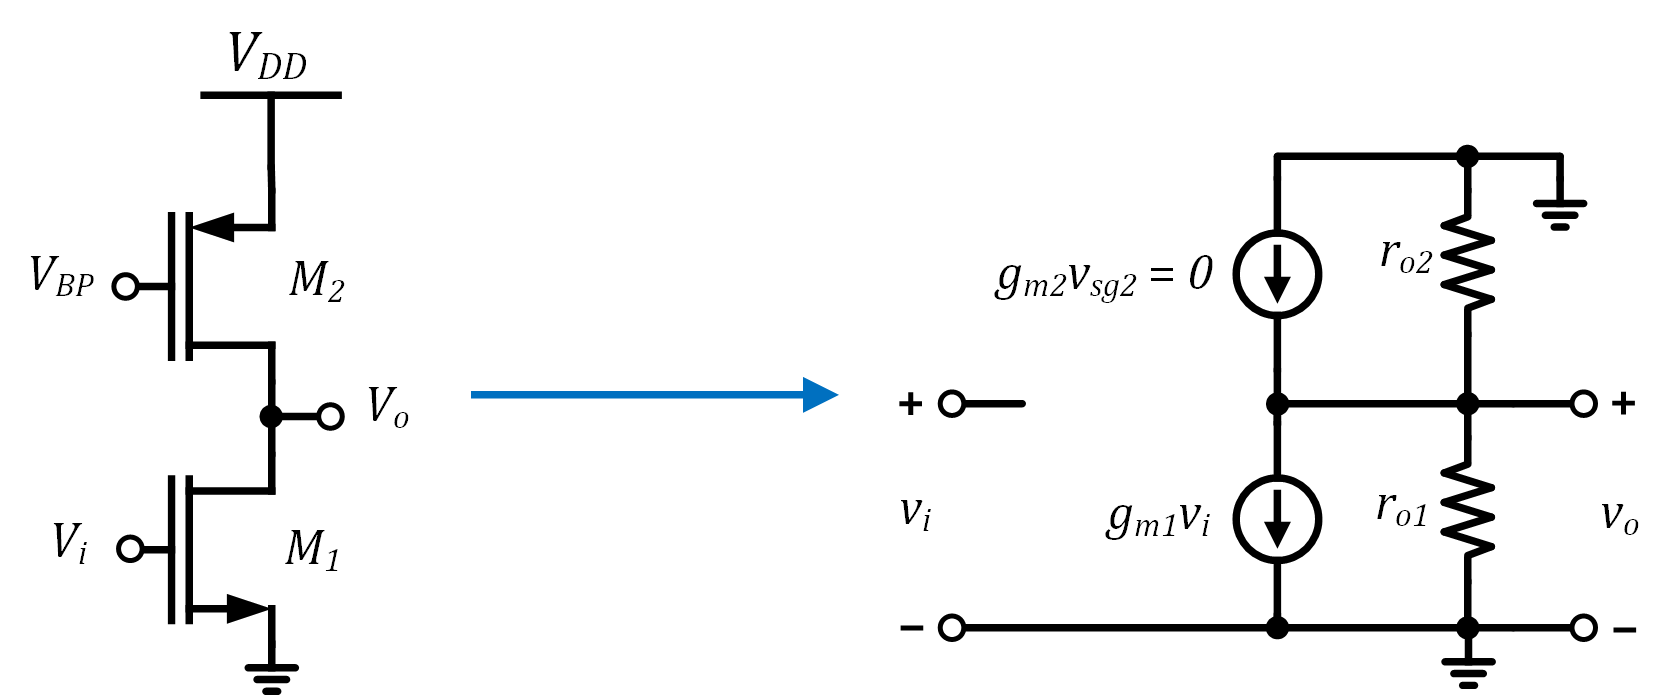
\includegraphics{common_source_active_small_signal.png}
\caption{common\_source\_active\_small\_signal.png}
\end{figure}

    \begin{itemize}
\tightlist
\item
  If the output voltage is maintained such that both \(M_1\) and \(M_2\)
  remain in saturation, the gain is determined by
\end{itemize}

\begin{equation}
A_v = \dfrac{v_o}{v_i} = -g_{m1}\cdot r_{o1}||r_{o2}
\end{equation}

\begin{itemize}
\tightlist
\item
  where \(g_{m1} = 2I_{D1}/V_{OV1}\), \(r_{o2} = 1/\lambda_n I_{D1}\),
  \(r_{o1} = 1/\lambda_p I_{D2}\), and \(I_{D1} = I_{D2}\)
\item
  \(I_{D2}\) (\(I_{D1}\)) constitutes the \(DC\) operating point of the
  circuit, and is often referred to as the ``bias current''
\item
  How do we control \(I_{D2}\)?
\end{itemize}

    \hypertarget{basic-current-mirror}{%
\subsection{Basic current mirror}\label{basic-current-mirror}}

    \begin{figure}
\centering
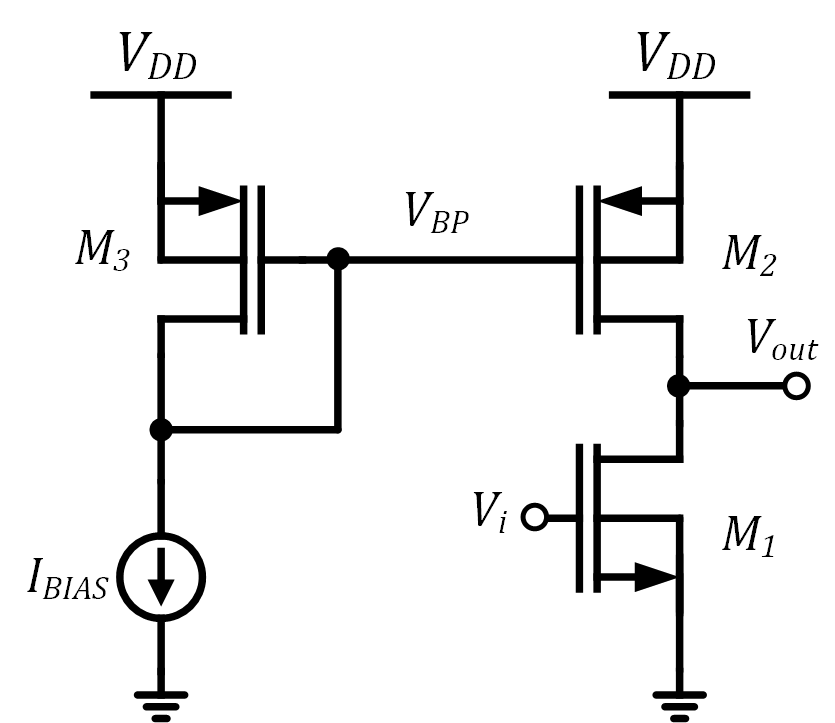
\includegraphics{common_source_biasing.png}
\caption{common\_source\_biasing.png}
\end{figure}

    \begin{itemize}
\tightlist
\item
  Assuming \(\lambda_p = 0\), if \((W/L)_2\) \$ = (W/L)\_3\$,
\end{itemize}

\begin{equation}
I_{D1} = I_{D2} = I_{D3} = I_{BIAS}
\end{equation}

\begin{itemize}
\tightlist
\item
  Hence,
\end{itemize}

\begin{equation}
g_{m1} = \dfrac{2I_{BIAS}}{V_{OV}}, \;\; r_{o1} = \dfrac{1}{\lambda_n I_{BIAS}}, \;\; r_{o2} = \dfrac{1}{\lambda_p I_{BIAS}} 
\end{equation}

    \begin{itemize}
\tightlist
\item
  A ``diode-connected'' transistor (\(M_3\) in the figure) converts a
  current (\(I_{BIAS}\)) into a voltage (\(V_{BP}\)) based on the
  relation
\item
  Current biasing in this manner allows us to control the small-signal
  performance of the circuit by designing \(I_{BIAS}\) to achieve
  specific goals (e.g.~gain, bandwidth, noise)
\end{itemize}

    \hypertarget{current-mirror-operation}{%
\subsection{Current mirror operation}\label{current-mirror-operation}}

    \begin{figure}
\centering
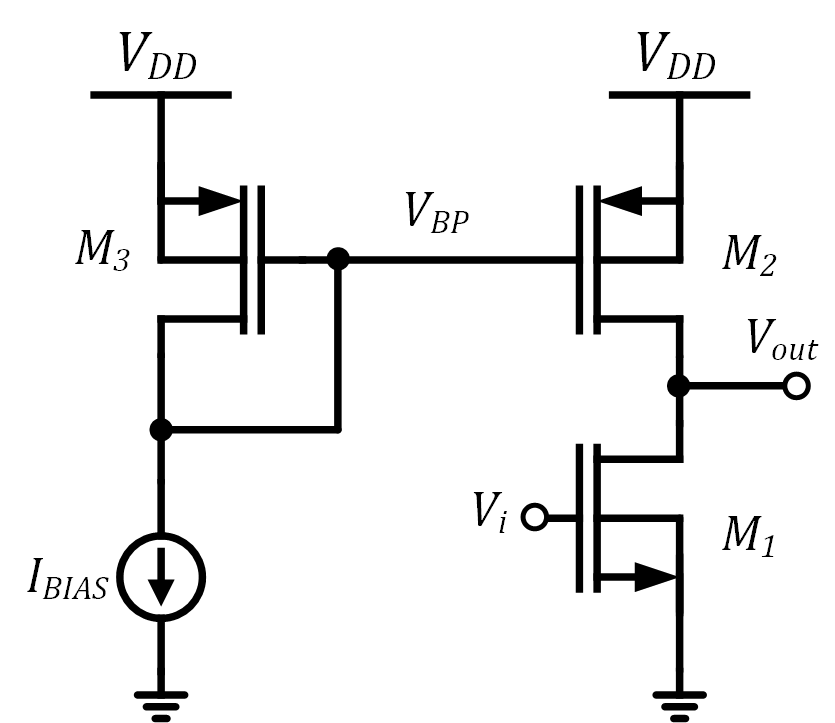
\includegraphics{common_source_biasing.png}
\caption{common\_source\_biasing.png}
\end{figure}

    \begin{itemize}
\tightlist
\item
  Again, assuming \(\lambda_p = 0\)
\end{itemize}

\begin{equation}
V_{SG3} = |V_{thp}| + \sqrt{\dfrac{2\cdot I_{BIAS}}{\mu_pC_{ox} \left(\dfrac{W}{L}\right)_3}}
\end{equation}

\begin{itemize}
\tightlist
\item
  The commmon-source bias current is thus
\end{itemize}

\begin{equation}
I_{D1} = I_{D2} = \dfrac{1}{2}\mu\cdot C_{ox} \cdot \dfrac{W}{L}(V_{DD}-V_{BP}-|V_{thp}|)^2
\end{equation}

    \begin{itemize}
\tightlist
\item
  The ``diode'' connection (gate and drain shorted together) ensures
  \(M_3\) is always in saturation, since
\end{itemize}

\begin{equation}
V_{SG} = V_{SD} > V_{SG} - |V_{thp}|
\end{equation}

\begin{itemize}
\tightlist
\item
  Because \(M_2\) and \(M_3\) share gate and source connections, \(M_2\)
  ``mirrors'' (i.e.~copies) \(M_3\)'s current
\item
  However, we have ignored the fact that \(V_{SD2}\) is not necessarily
  equal to \(V_{SD3}\)
\item
  How do \(I_{D1}\), \(I_{D2}\) vary with \(V_{out}\)?
\end{itemize}

    \hypertarget{finite-output-resistance}{%
\subsection{Finite output resistance}\label{finite-output-resistance}}

    \begin{figure}
\centering
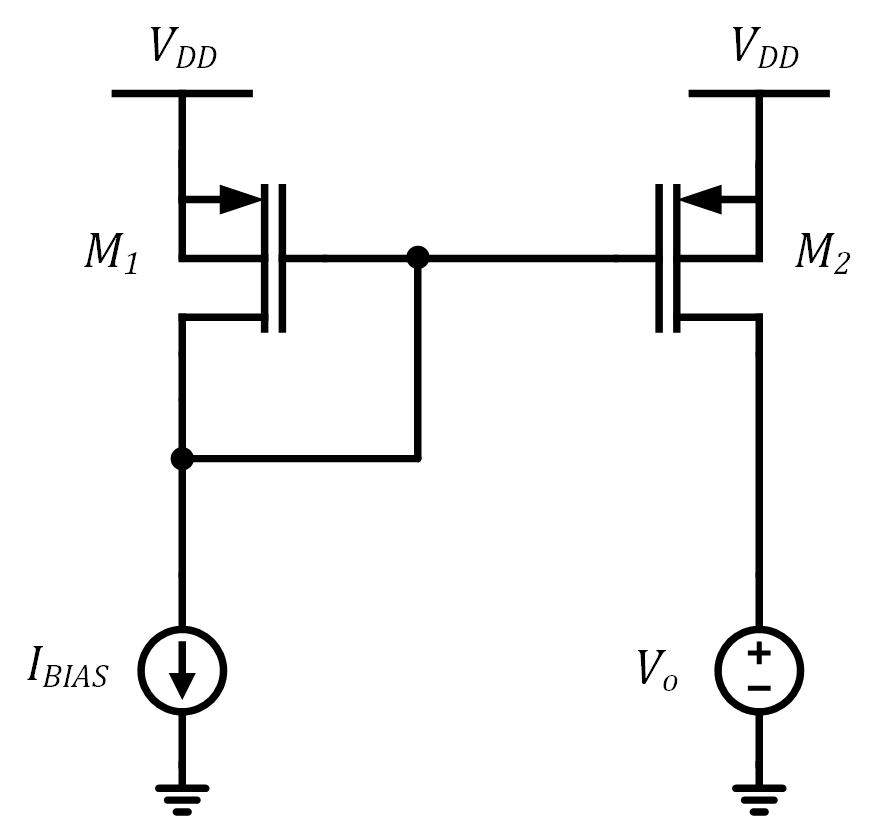
\includegraphics{current_mirror_output_resistance.png}
\caption{current\_mirror\_output\_resistance.png}
\end{figure}

    \begin{itemize}
\tightlist
\item
  Considering the effect of channel-length modulation on \(M_2\)'s drain
  current gives
\end{itemize}

\begin{equation}
I_{D2} = \dfrac{1}{2}\mu\cdot C_{ox} \cdot \dfrac{W}{L}(V_{DD}-V_{BP}-|V_{thp}|)^2[1+\lambda (V_{DD} - V_o) ]
\end{equation}

\begin{itemize}
\tightlist
\item
  To assess the dependence of \(I_{D2}\) on \(V_o\), we can take the
  derivative
\end{itemize}

\begin{equation}
\dfrac{\partial I_{D2}}{\partial V_o} = \dfrac{1}{r_{o2}}
\end{equation}

    \begin{itemize}
\tightlist
\item
  The purpose of \(M_2\) is to provide current for the common-source
  stage
\item
  The output resistance of the current mirror captures the dependence of
  \(I_{D2}\), which determines \emph{how} effectively it operates as a
  current source
\item
  It turns out then that the same factor limiting voltage gain in the
  common-source stage limits the precision of a current mirror:
  \emph{output resistance}
\item
  How can we increase output resistance and, as a result, gain?
\item
  More on this next time\ldots{}
\end{itemize}

    \hypertarget{summary}{%
\subsection{Summary}\label{summary}}

    \begin{itemize}
\tightlist
\item
  High gain in operational amplifiers (Opamps) and operational
  \emph{transconductance} amplifiers (OTAs) is achieved using (one or
  more) structures similar in form to the common-source stage

  \begin{itemize}
  \tightlist
  \item
    Voltage gain is realized as the product of a transconductance
    (\(G_m\)) and a resistance (\(R_o\))
  \end{itemize}
\item
  Active loads enable higher values of \(R_o\), and thus higher gain,
  than passive loads
\item
  Current biasing allows us to precisely define the critical
  small-signal parameters (\(g_m\), \(r_o\)) that determine circuit
  performance
\item
  Finite MOS output resistance limits both gain and the precision of
  current mirrors
\item
  Next time, we will look at how to build both better current mirrors
  and voltage amplification stages
\end{itemize}


    % Add a bibliography block to the postdoc
    
    
    
\end{document}
